% ----------------------------------------------------------------------
%
%                            TFMTesis.tex
%
%----------------------------------------------------------------------
%
% Este fichero contiene el "documento maestro" del documento. Lo único
% que hace es configurar el entorno LaTeX e incluir los ficheros .tex
% que contienen cada sección.
%
%----------------------------------------------------------------------
%
% Los ficheros necesarios para este documento son:
%
%       TeXiS/* : ficheros de la plantilla TeXiS.
%       Cascaras/* : ficheros con las partes del documento que no
%          son capítulos ni apéndices (portada, agradecimientos, etc.)
%       Capitulos/*.tex : capítulos de la tesis
%       Apendices/*.tex: apéndices de la tesis
%       constantes.tex: constantes LaTeX
%       config.tex : configuración de la "compilación" del documento
%       guionado.tex : palabras con guiones
%
% Para la bibliografía, además, se necesitan:
%
%       *.bib : ficheros con la información de las referencias
%
% ---------------------------------------------------------------------

\documentclass[12pt,a4paper,oneside]{book}

%
% Definimos  el   comando  \compilaCapitulo,  que   luego  se  utiliza
% (opcionalmente) en config.tex. Quedaría  mejor si también se definiera
% en  ese fichero,  pero por  el modo  en el  que funciona  eso  no es
% posible. Puedes consultar la documentación de ese fichero para tener
% más  información. Definimos también  \compilaApendice, que  tiene el
% mismo  cometido, pero  que se  utiliza para  compilar  únicamente un
% apéndice.
%
%
% Si  queremos   compilar  solo   una  parte  del   documento  podemos
% especificar mediante  \includeonly{...} qué ficheros  son los únicos
% que queremos  que se incluyan.  Esto  es útil por  ejemplo para sólo
% compilar un capítulo.
%
% El problema es que todos aquellos  ficheros que NO estén en la lista
% NO   se  incluirán...  y   eso  también   afecta  a   ficheros  de
% la plantilla...
%
% Total,  que definimos  una constante  con los  ficheros  que siempre
% vamos a querer compilar  (aquellos relacionados con configuración) y
% luego definimos \compilaCapitulo.
\newcommand{\ficherosBasicosTeXiS}{%
TeXiS/TeXiS_pream,TeXiS/TeXiS_cab,TeXiS/TeXiS_bib,TeXiS/TeXiS_cover%
}
\newcommand{\ficherosBasicosTexto}{%
constantes,guionado,Cascaras/bibliografia,config%
}
\newcommand{\compilaCapitulo}[1]{%
\includeonly{\ficherosBasicosTeXiS,\ficherosBasicosTexto,Capitulos/#1}%
}

\newcommand{\compilaApendice}[1]{%
\includeonly{\ficherosBasicosTeXiS,\ficherosBasicosTexto,Apendices/#1}%
}

%- - - - - - - - - - - - - - - - - - - - - - - - - - - - - - - - - - -
%            Preámbulo del documento. Configuraciones varias
%- - - - - - - - - - - - - - - - - - - - - - - - - - - - - - - - - - -

% Define  el  tipo  de  compilación que  estamos  haciendo.   Contiene
% definiciones  de  constantes que  cambian  el  comportamiento de  la
% compilación. Debe incluirse antes del paquete TeXiS/TeXiS.sty
%---------------------------------------------------------------------
%
%                          config.tex
%
%---------------------------------------------------------------------
%
% Contiene la  definición de constantes  que determinan el modo  en el
% que se compilará el documento.
%
%---------------------------------------------------------------------
%
% En concreto, podemos  indicar si queremos "modo release",  en el que
% no  aparecerán  los  comentarios  (creados  mediante  \com{Texto}  o
% \comp{Texto}) ni los "por  hacer" (creados mediante \todo{Texto}), y
% sí aparecerán los índices. El modo "debug" (o mejor dicho en modo no
% "release" muestra los índices  (construirlos lleva tiempo y son poco
% útiles  salvo  para   la  versión  final),  pero  sí   el  resto  de
% anotaciones.
%
% Si se compila con LaTeX (no  con pdflatex) en modo Debug, también se
% muestran en una esquina de cada página las entradas (en el índice de
% palabras) que referencian  a dicha página (consulta TeXiS_pream.tex,
% en la parte referente a show).
%
% El soporte para  el índice de palabras en  TeXiS es embrionario, por
% lo  que no  asumas que  esto funcionará  correctamente.  Consulta la
% documentación al respecto en TeXiS_pream.tex.
%
%
% También  aquí configuramos  si queremos  o  no que  se incluyan  los
% acrónimos  en el  documento final  en la  versión release.  Para eso
% define (o no) la constante \acronimosEnRelease.
%
% Utilizando \compilaCapitulo{nombre}  podemos también especificar qué
% capítulo(s) queremos que se compilen. Si no se pone nada, se compila
% el documento  completo.  Si se pone, por  ejemplo, 01Introduccion se
% compilará únicamente el fichero Capitulos/01Introduccion.tex
%
% Para compilar varios  capítulos, se separan sus nombres  con comas y
% no se ponen espacios de separación.
%
% En realidad  la macro \compilaCapitulo  está definida en  el fichero
% principal tesis.tex.
%
%---------------------------------------------------------------------


% Comentar la línea si no se compila en modo release.
% TeXiS hará el resto.
% ¡¡¡Si cambias esto, haz un make clean antes de recompilar!!!
\def\release{1}


% Descomentar la linea si se quieren incluir los
% acrónimos en modo release (en modo debug
% no se incluirán nunca).
% ¡¡¡Si cambias esto, haz un make clean antes de recompilar!!!
% \def\acronimosEnRelease{1}


% Descomentar la línea para establecer el capítulo que queremos
% compilar

% \compilaCapitulo{01Introduccion}
% \compilaCapitulo{02EstructuraYGeneracion}
% \compilaCapitulo{03Edicion}
% \compilaCapitulo{04Imagenes}
% \compilaCapitulo{05Bibliografia}
% \compilaCapitulo{06Makefile}

% \compilaApendice{01AsiSeHizo}

% Variable local para emacs, para  que encuentre el fichero maestro de
% compilación y funcionen mejor algunas teclas rápidas de AucTeX
%%%
%%% Local Variables:
%%% mode: latex
%%% TeX-master: "./Tesis.tex"
%%% End:


% Paquete de la plantilla
\usepackage{TeXiS/TeXiS}

% Incluimos el fichero con comandos de constantes
%---------------------------------------------------------------------
%
%                          constantes.tex
%
%---------------------------------------------------------------------
%
% Fichero que  declara nuevos comandos LaTeX  sencillos realizados por
% comodidad en la escritura de determinadas palabras
%
%---------------------------------------------------------------------

%%%%%%%%%%%%%%%%%%%%%%%%%%%%%%%%%%%%%%%%%%%%%%%%%%%%%%%%%%%%%%%%%%%%%%
% Comando: 
%
%       \titulo
%
% Resultado: 
%
% Escribe el título del documento.
%%%%%%%%%%%%%%%%%%%%%%%%%%%%%%%%%%%%%%%%%%%%%%%%%%%%%%%%%%%%%%%%%%%%%%
\def\titulo{Desarrollo de una app movil para gestionar servicios de expertos profesionales}

%%%%%%%%%%%%%%%%%%%%%%%%%%%%%%%%%%%%%%%%%%%%%%%%%%%%%%%%%%%%%%%%%%%%%%
% Comando: 
%
%       \autor
%
% Resultado: 
%
% Escribe el autor del documento.
%%%%%%%%%%%%%%%%%%%%%%%%%%%%%%%%%%%%%%%%%%%%%%%%%%%%%%%%%%%%%%%%%%%%%%
\def\autor{Jaime Pablo V\'azquez Mart\'in}

% Variable local para emacs, para  que encuentre el fichero maestro de
% compilación y funcionen mejor algunas teclas rápidas de AucTeX

%%%
%%% Local Variables:
%%% mode: latex
%%% TeX-master: "tesis.tex"
%%% End:


% Sacamos en el log de la compilación el copyright
%\typeout{Copyright Marco Antonio and Pedro Pablo Gomez Martin}

%
% "Metadatos" para el PDF
%
\ifpdf\hypersetup{%
    pdftitle = {\titulo},
    pdfsubject = {trabajo de fin de grado},
    pdfkeywords = {Plantilla, LaTeX, trabajo de grado},
    pdfauthor = {\textcopyright\ \autor},
    pdfcreator = {\LaTeX\ con el paquete \flqq hyperref\frqq},
    pdfproducer = {pdfeTeX-0.\the\pdftexversion\pdftexrevision},
    }
    \pdfinfo{/CreationDate (\today)}
\fi


%- - - - - - - - - - - - - - - - - - - - - - - - - - - - - - - - - - -
%                        Documento
%- - - - - - - - - - - - - - - - - - - - - - - - - - - - - - - - - - -
\begin{document}

% Incluimos el  fichero de definición de guionado  de algunas palabras
% que LaTeX no ha dividido como debería
%----------------------------------------------------------------
%
%                          guionado.tex
%
%----------------------------------------------------------------
%
% Fichero con algunas divisiones de palabras que LaTeX no
% hace correctamente si no se le da alguna ayuda.
%
%----------------------------------------------------------------

\hyphenation{
% a
abs-trac-to
abs-trac-tos
abs-trac-ta
abs-trac-tas
ac-tua-do-res
a-gra-de-ci-mien-tos
ana-li-za-dor
an-te-rio-res
an-te-rior-men-te
apa-rien-cia
a-pro-pia-do
a-pro-pia-dos
a-pro-pia-da
a-pro-pia-das
a-pro-ve-cha-mien-to
a-que-llo
a-que-llos
a-que-lla
a-que-llas
a-sig-na-tu-ra
a-sig-na-tu-ras
a-so-cia-da
a-so-cia-das
a-so-cia-do
a-so-cia-dos
au-to-ma-ti-za-do
% b
batch
bi-blio-gra-fía
bi-blio-grá-fi-cas
bien
bo-rra-dor
boo-l-ean-expr
% c
ca-be-ce-ra
call-me-thod-ins-truc-tion
cas-te-lla-no
cir-cuns-tan-cia
cir-cuns-tan-cias
co-he-ren-te
co-he-ren-tes
co-he-ren-cia
co-li-bri
co-men-ta-rio
co-mer-cia-les
co-no-ci-mien-to
cons-cien-te
con-si-de-ra-ba
con-si-de-ra-mos
con-si-de-rar-se
cons-tan-te
cons-trucción
cons-tru-ye
cons-tru-ir-se
con-tro-le
co-rrec-ta-men-te
co-rres-pon-den
co-rres-pon-dien-te
co-rres-pon-dien-tes
co-ti-dia-na
co-ti-dia-no
crean
cris-ta-li-zan
cu-rri-cu-la
cu-rri-cu-lum
cu-rri-cu-lar
cu-rri-cu-la-res
% d
de-di-ca-do
de-di-ca-dos
de-di-ca-da
de-di-ca-das
de-rro-te-ro
de-rro-te-ros
de-sa-rro-llo
de-sa-rro-llos
de-sa-rro-lla-do
de-sa-rro-lla-dos
de-sa-rro-lla-da
de-sa-rro-lla-das
de-sa-rro-lla-dor
de-sa-rro-llar
des-cri-bi-re-mos
des-crip-ción
des-crip-cio-nes
des-cri-to
des-pués
de-ta-lla-do
de-ta-lla-dos
de-ta-lla-da
de-ta-lla-das
di-a-gra-ma
di-a-gra-mas
di-se-ños
dis-po-ner
dis-po-ni-bi-li-dad
do-cu-men-ta-da
do-cu-men-to
do-cu-men-tos
% e
edi-ta-do
e-du-ca-ti-vo
e-du-ca-ti-vos
e-du-ca-ti-va
e-du-ca-ti-vas
e-la-bo-ra-do
e-la-bo-ra-dos
e-la-bo-ra-da
e-la-bo-ra-das
es-co-llo
es-co-llos
es-tu-dia-do
es-tu-dia-dos
es-tu-dia-da
es-tu-dia-das
es-tu-dian-te
e-va-lua-cio-nes
e-va-lua-do-res
exis-ten-tes
exhaus-ti-va
ex-pe-rien-cia
ex-pe-rien-cias
% f
for-ma-li-za-do
% g
ge-ne-ra-ción
ge-ne-ra-dor
ge-ne-ra-do-res
ge-ne-ran
% h
he-rra-mien-ta
he-rra-mien-tas
% i
i-dio-ma
i-dio-mas
im-pres-cin-di-ble
im-pres-cin-di-bles
in-de-xa-do
in-de-xa-dos
in-de-xa-da
in-de-xa-das
in-di-vi-dual
in-fe-ren-cia
in-fe-ren-cias
in-for-ma-ti-ca
in-gre-dien-te
in-gre-dien-tes
in-me-dia-ta-men-te
ins-ta-la-do
ins-tan-cias
% j
% k
% l
len-gua-je
li-be-ra-to-rio
li-be-ra-to-rios
li-be-ra-to-ria
li-be-ra-to-rias
li-mi-ta-do
li-te-ra-rio
li-te-ra-rios
li-te-ra-ria
li-te-ra-rias
lo-tes
% m
ma-ne-ra
ma-nual
mas-que-ra-de
ma-yor
me-mo-ria
mi-nis-te-rio
mi-nis-te-rios
mo-de-lo
mo-de-los
mo-de-la-do
mo-du-la-ri-dad
mo-vi-mien-to
% n
na-tu-ral
ni-vel
nues-tro
% o
obs-tan-te
o-rien-ta-do
o-rien-ta-dos
o-rien-ta-da
o-rien-ta-das
% p
pa-ra-le-lo
pa-ra-le-la
par-ti-cu-lar
par-ti-cu-lar-men-te
pe-da-gó-gi-ca
pe-da-gó-gi-cas
pe-da-gó-gi-co
pe-da-gó-gi-cos
pe-rio-di-ci-dad
per-so-na-je
plan-te-a-mien-to
plan-te-a-mien-tos
po-si-ción
pre-fe-ren-cia
pre-fe-ren-cias
pres-cin-di-ble
pres-cin-di-bles
pri-me-ra
pro-ble-ma
pro-ble-mas
pró-xi-mo
pu-bli-ca-cio-nes
pu-bli-ca-do
% q
% r
rá-pi-da
rá-pi-do
ra-zo-na-mien-to
ra-zo-na-mien-tos
re-a-li-zan-do
re-fe-ren-cia
re-fe-ren-cias
re-fe-ren-cia-da
re-fe-ren-cian
re-le-van-tes
re-pre-sen-ta-do
re-pre-sen-ta-dos
re-pre-sen-ta-da
re-pre-sen-ta-das
re-pre-sen-tar-lo
re-qui-si-to
re-qui-si-tos
res-pon-der
res-pon-sa-ble
% s
se-pa-ra-do
si-guien-do
si-guien-te
si-guien-tes
si-guie-ron
si-mi-lar
si-mi-la-res
si-tua-ción
% t
tem-pe-ra-ments
te-ner
trans-fe-ren-cia
trans-fe-ren-cias
% u
u-sua-rio
Unreal-Ed
% v
va-lor
va-lo-res
va-rian-te
ver-da-de-ro
ver-da-de-ros
ver-da-de-ra
ver-da-de-ras
ver-da-de-ra-men-te
ve-ri-fi-ca
% w
% x
% y
% z
}
% Variable local para emacs, para que encuentre el fichero
% maestro de compilación
%%%
%%% Local Variables:
%%% mode: latex
%%% TeX-master: "./Tesis.tex"
%%% End:


% Marcamos  el inicio  del  documento para  la  numeración de  páginas
% (usando números romanos para esta primera fase).
\frontmatter
\pagestyle{empty}

%---------------------------------------------------------------------
%
%                          configCover.tex
%
%---------------------------------------------------------------------
%
% cover.tex
% Copyright 2009 Marco Antonio Gomez-Martin, Pedro Pablo Gomez-Martin
%
% This file belongs to the TeXiS manual, a LaTeX template for writting
% Thesis and other documents. The complete last TeXiS package can
% be obtained from http://gaia.fdi.ucm.es/projects/texis/
%
% Although the TeXiS template itself is distributed under the 
% conditions of the LaTeX Project Public License
% (http://www.latex-project.org/lppl.txt), the manual content
% uses the CC-BY-SA license that stays that you are free:
%
%    - to share & to copy, distribute and transmit the work
%    - to remix and to adapt the work
%
% under the following conditions:
%
%    - Attribution: you must attribute the work in the manner
%      specified by the author or licensor (but not in any way that
%      suggests that they endorse you or your use of the work).
%    - Share Alike: if you alter, transform, or build upon this
%      work, you may distribute the resulting work only under the
%      same, similar or a compatible license.
%
% The complete license is available in
% http://creativecommons.org/licenses/by-sa/3.0/legalcode
%
%---------------------------------------------------------------------
%
% Fichero que contiene la configuración de la portada y de la 
% primera hoja del documento.
%
%---------------------------------------------------------------------


% Pueden configurarse todos los elementos del contenido de la portada
% utilizando comandos.

%%%%%%%%%%%%%%%%%%%%%%%%%%%%%%%%%%%%%%%%%%%%%%%%%%%%%%%%%%%%%%%%%%%%%%
% Título del documento:
% \tituloPortada{titulo}
% Nota:
% Si no se define se utiliza el del \titulo. Este comando permite
% cambiar el título de forma que se especifiquen dónde se quieren
% los retornos de carro cuando se utilizan fuentes grandes.
%%%%%%%%%%%%%%%%%%%%%%%%%%%%%%%%%%%%%%%%%%%%%%%%%%%%%%%%%%%%%%%%%%%%%%
\tituloPortada{%
    \titulo
}


%%%%%%%%%%%%%%%%%%%%%%%%%%%%%%%%%%%%%%%%%%%%%%%%%%%%%%%%%%%%%%%%%%%%%%
% Título del documento en inglés:
% \tituloPortadaEng{titulo}
% Nota:
% Si no se define se utiliza el del \titulo. Este comando permite
% cambiar el título de forma que se especifiquen dónde se quieren
% los retornos de carro cuando se utilizan fuentes grandes.
%%%%%%%%%%%%%%%%%%%%%%%%%%%%%%%%%%%%%%%%%%%%%%%%%%%%%%%%%%%%%%%%%%%%%%
\tituloPortadaEng{%
    Profinder: a mobile app to manage professional expert's services
}

%%%%%%%%%%%%%%%%%%%%%%%%%%%%%%%%%%%%%%%%%%%%%%%%%%%%%%%%%%%%%%%%%%%%%%
% Autor del documento:
% \autorPortada{Nombre}
% Se utiliza en la portada y en el valor por defecto del
% primer subtítulo de la segunda portada.
%%%%%%%%%%%%%%%%%%%%%%%%%%%%%%%%%%%%%%%%%%%%%%%%%%%%%%%%%%%%%%%%%%%%%%
\autorPortada{
    \autor
}

%%%%%%%%%%%%%%%%%%%%%%%%%%%%%%%%%%%%%%%%%%%%%%%%%%%%%%%%%%%%%%%%%%%%%%
% Fecha de publicación:
% \fechaPublicacion{Fecha}
% Puede ser vacío. Aparece en la última línea de ambas portadas
%%%%%%%%%%%%%%%%%%%%%%%%%%%%%%%%%%%%%%%%%%%%%%%%%%%%%%%%%%%%%%%%%%%%%%
% Descomentar para que ponga siempre la fecha actual
%\fechaPublicacion{\today}
\fechaPublicacion{27 de Mayo de 2024}

%%%%%%%%%%%%%%%%%%%%%%%%%%%%%%%%%%%%%%%%%%%%%%%%%%%%%%%%%%%%%%%%%%%%%%
% Imagen de la portada (y escala)
% \imagenPortada{Fichero}
% \escalaImagenPortada{Numero}
% Si no se especifica, se utiliza la imagen TODO.pdf
%%%%%%%%%%%%%%%%%%%%%%%%%%%%%%%%%%%%%%%%%%%%%%%%%%%%%%%%%%%%%%%%%%%%%%
% imagen en blanco y negro
%\imagenPortada{Imagenes/Vectorial/escudoUCM}
%imagen en color
\imagenPortada{Imagenes/Bitmap/escudoUCMcolor}
\escalaImagenPortada{.2}

%%%%%%%%%%%%%%%%%%%%%%%%%%%%%%%%%%%%%%%%%%%%%%%%%%%%%%%%%%%%%%%%%%%%%%
% Tipo de documento.
% \tipoDocumento{Tipo}
% Para el texto justo debajo del escudo.
% Si no se indica, se utiliza "TESIS DOCTORAL".
%%%%%%%%%%%%%%%%%%%%%%%%%%%%%%%%%%%%%%%%%%%%%%%%%%%%%%%%%%%%%%%%%%%%%%
\tipoDocumento{Trabajo de Fin de Grado}

%%%%%%%%%%%%%%%%%%%%%%%%%%%%%%%%%%%%%%%%%%%%%%%%%%%%%%%%%%%%%%%%%%%%%%
% Institución/departamento asociado al documento.
% \institucion{Nombre}
% Puede tener varias líneas. Se utiliza en las dos portadas.
% Si no se indica aparecerá vacío.
%%%%%%%%%%%%%%%%%%%%%%%%%%%%%%%%%%%%%%%%%%%%%%%%%%%%%%%%%%%%%%%%%%%%%%
\institucion{%
Grado en Ingeniería Informática\\[0.2em]
Facultad de Informática\\[0.2em]
Universidad Complutense de Madrid
}

%%%%%%%%%%%%%%%%%%%%%%%%%%%%%%%%%%%%%%%%%%%%%%%%%%%%%%%%%%%%%%%%%%%%%%
% Director del trabajo.
% \directorPortada{Nombre}
% Se utiliza para el valor por defecto del segundo subtítulo, donde
% se indica quién es el director del trabajo.
% Si se fuerza un subtítulo distinto, no hace falta definirlo.
%%%%%%%%%%%%%%%%%%%%%%%%%%%%%%%%%%%%%%%%%%%%%%%%%%%%%%%%%%%%%%%%%%%%%%
\directorPortada{Antonio Sarasa Cabezuelo}


%%%%%%%%%%%%%%%%%%%%%%%%%%%%%%%%%%%%%%%%%%%%%%%%%%%%%%%%%%%%%%%%%%%%%%
% Colaborador en la dirección del trabajo.
% \colaboradorPortada{Nombre}
% Se utiliza para el valor por defecto del segundo subtítulo, donde
% se indica quién es el colaborador en la dirección del trabajo.
% Si se fuerza un subtítulo distinto, no hace falta definirlo.
%%%%%%%%%%%%%%%%%%%%%%%%%%%%%%%%%%%%%%%%%%%%%%%%%%%%%%%%%%%%%%%%%%%%%%
% \colaboradorPortada{\textcolor{red}{Colaborador 1\\Colaborador 2}}


%%%%%%%%%%%%%%%%%%%%%%%%%%%%%%%%%%%%%%%%%%%%%%%%%%%%%%%%%%%%%%%%%%%%%%
% Texto del primer subtítulo de la segunda portada.
% \textoPrimerSubtituloPortada{Texto}
% Para configurar el primer "texto libre" de la segunda portada.
% Si no se especifica se indica "Memoria que presenta para optar al
% título de Doctor en Informática" seguido del \autorPortada.
%%%%%%%%%%%%%%%%%%%%%%%%%%%%%%%%%%%%%%%%%%%%%%%%%%%%%%%%%%%%%%%%%%%%%%
\textoPrimerSubtituloPortada{%
\textbf{Trabajo de Fin de Grado en Ingeniería Informática}\\ [0.3em]
}

%%%%%%%%%%%%%%%%%%%%%%%%%%%%%%%%%%%%%%%%%%%%%%%%%%%%%%%%%%%%%%%%%%%%%%
% Texto del segundo subtítulo de la segunda portada.
% \textoSegundoSubtituloPortada{Texto}
% Para configurar el segundo "texto libre" de la segunda portada.
% Si no se especifica se indica "Dirigida por el Doctor" seguido
% del \directorPortada.
%%%%%%%%%%%%%%%%%%%%%%%%%%%%%%%%%%%%%%%%%%%%%%%%%%%%%%%%%%%%%%%%%%%%%%
\textoSegundoSubtituloPortada{%
\textbf{Convocatoria: }\textit{Junio \the\year}%\\[0.2em]
%\textbf{Calificación: }\textit{\textcolor{red}{Nota}}
}

%%%%%%%%%%%%%%%%%%%%%%%%%%%%%%%%%%%%%%%%%%%%%%%%%%%%%%%%%%%%%%%%%%%%%%
% \explicacionDobleCara
% Si se utiliza, se aclara que el documento está preparado para la
% impresión a doble cara.
%%%%%%%%%%%%%%%%%%%%%%%%%%%%%%%%%%%%%%%%%%%%%%%%%%%%%%%%%%%%%%%%%%%%%%
%\explicacionDobleCara

%%%%%%%%%%%%%%%%%%%%%%%%%%%%%%%%%%%%%%%%%%%%%%%%%%%%%%%%%%%%%%%%%%%%%%
% \isbn
% Si se utiliza, aparecerá el ISBN detrás de la segunda portada.
%%%%%%%%%%%%%%%%%%%%%%%%%%%%%%%%%%%%%%%%%%%%%%%%%%%%%%%%%%%%%%%%%%%%%%
%\isbn{978-84-692-7109-4}


%%%%%%%%%%%%%%%%%%%%%%%%%%%%%%%%%%%%%%%%%%%%%%%%%%%%%%%%%%%%%%%%%%%%%%
% \copyrightInfo
% Si se utiliza, aparecerá información de los derechos de copyright
% detrás de la segunda portada.
%%%%%%%%%%%%%%%%%%%%%%%%%%%%%%%%%%%%%%%%%%%%%%%%%%%%%%%%%%%%%%%%%%%%%%
%\copyrightInfo{\autor}


%%
%% Creamos las portadas
%%
\makeCover

% Variable local para emacs, para que encuentre el fichero
% maestro de compilación
%%%
%%% Local Variables:
%%% mode: latex
%%% TeX-master: "../Tesis.tex"
%%% End:

%\include{Cascaras/autorizacion}
% +--------------------------------------------------------------------+
% | Dedication Page (Optional)
% +--------------------------------------------------------------------+

\chapter*{Dedicatoria}

\begin{flushright}
\begin{minipage}[c]{8.5cm}
\flushright{\textit{A mis padres Pablo y Elena por apoyarme y ayudarme siempre. Sin ellos nada de esto habría sido posible.}}
\end{minipage}
\end{flushright}
% +--------------------------------------------------------------------+
% | Acknowledgements Page (Optional)                                   |
% +--------------------------------------------------------------------+

\chapter*{Agradecimientos}

A Antonio Sarasa, mi tutor, por estar siempre disponible. A Jorge Roselló, que me ayudó a iniciarme en lo que ha sido y será mi viaje en el mundo del desarrollo Android. A Aristides Guimerá (Aristidevs), creador de contenido online sin cuyos vídeos y cursos no habría avanzado tan comodamente en mi proceso de aprendizaje. Y a Marco Antonio Gómez Martín y Pedro Pablo Gómez Martín por facilitar esta plantilla tan útil.












\chapter*{Resumen}

\section*{\tituloPortadaVal}

Profinder es una aplicación que ha sido desarrollada para dispositivos con sistema operativo Android. Busca ser un sistema que ayude a profesionales de distintos campos a ponerse en contacto con nuevos clientes, mantener conversaciones con ellos y crear una reputación mediante la calificación que los clientes creen al terminar los servicios realizados por el profesional, a su vez los clientes serán calificados por los profesionales. Los usuarios podrán utilizar la funcionalidad de mapa para comprobar qué profesionales están trabajando por la zona, agilizando así los tiempos de espera. Tanto profesionales como clientes podrán ser agregados a una lista de favoritos para tener fácil acceso a estos si fuera necesario. Tanto profesionales como servicios estarán clasificados dentro de categorías que permitirán una mejor gestión y organización.

La aplicación ha sido desarrollada siguiendo las mejores prácticas posibles, tanto a nivel de código como de arquitectura. Se ha utilizado kotlin como lenguaje de programación de la aplicación (más moderno, seguro, y eficiente que java). Para las interfaces se ha utilizado el kit de herramientas de Jetpack Compose diseñado para simplificar el desarrollo de IU.

\section*{Palabras clave}
   
\noindent profesional, usuario, servicio, mapa, chat, favoritos, categoría, android.

   



\begin{otherlanguage}{english}
\chapter*{Abstract}

\section*{\tituloPortadaEngVal}

An abstract in English, half a page long, including the title in English. Below, a list with no more than 10 keywords.


\section*{Keywords}

\noindent 10 keywords max., separated by commas.




% Si el trabajo se escribe en inglés, comentar esta línea y descomentar
% otra igual que hay justo antes de \end{document}
\end{otherlanguage}

\ifx\generatoc\undefined
\else
%---------------------------------------------------------------------
%
%                          TeXiS_toc.tex
%
%---------------------------------------------------------------------
%
% TeXiS_toc.tex
% Copyright 2009 Marco Antonio Gomez-Martin, Pedro Pablo Gomez-Martin
%
% This file belongs to TeXiS, a LaTeX template for writting
% Thesis and other documents. The complete last TeXiS package can
% be obtained from http://gaia.fdi.ucm.es/projects/texis/
%
% This work may be distributed and/or modified under the
% conditions of the LaTeX Project Public License, either version 1.3
% of this license or (at your option) any later version.
% The latest version of this license is in
%   http://www.latex-project.org/lppl.txt
% and version 1.3 or later is part of all distributions of LaTeX
% version 2005/12/01 or later.
%
% This work has the LPPL maintenance status `maintained'.
% 
% The Current Maintainers of this work are Marco Antonio Gomez-Martin
% and Pedro Pablo Gomez-Martin
%
%---------------------------------------------------------------------
%
% Contiene  los  comandos  para  generar los  índices  del  documento,
% entendiendo por índices las tablas de contenidos.
%
% Genera  el  índice normal  ("tabla  de  contenidos"),  el índice  de
% figuras y el de tablas. También  crea "marcadores" en el caso de que
% se esté compilando con pdflatex para que aparezcan en el PDF.
%
%---------------------------------------------------------------------


% Primero un poquito de configuración...


% Pedimos que inserte todos los epígrafes hasta el nivel \subsection en
% la tabla de contenidos.
\setcounter{tocdepth}{2} 

% Le  pedimos  que nos  numere  todos  los  epígrafes hasta  el  nivel
% \subsubsection en el cuerpo del documento.
\setcounter{secnumdepth}{3} 


% Creamos los diferentes índices.

% Lo primero un  poco de trabajo en los marcadores  del PDF. No quiero
% que  salga una  entrada  por cada  índice  a nivel  0...  si no  que
% aparezca un marcador "Índices", que  tenga dentro los otros tipos de
% índices.  Total, que creamos el marcador "Índices".
% Antes de  la creación  de los índices,  se añaden los  marcadores de
% nivel 1.

\ifpdf
   \pdfbookmark{Índices}{indices}
\fi

% Tabla de contenidos.
%
% La  inclusión  de '\tableofcontents'  significa  que  en la  primera
% pasada  de  LaTeX  se  crea   un  fichero  con  extensión  .toc  con
% información sobre la tabla de contenidos (es conceptualmente similar
% al  .bbl de  BibTeX, creo).  En la  segunda ejecución  de  LaTeX ese
% documento se utiliza para  generar la verdadera página de contenidos
% usando la  información sobre los  capítulos y demás guardadas  en el
% .toc
\ifpdf
   \pdfbookmark[1]{Tabla de Contenidos}{tabla de contenidos}
\fi

\cabeceraEspecial{\'Indice}

\tableofcontents

\newpage 

% Índice de figuras
%
% La idea es semejante que para  el .toc del índice, pero ahora se usa
% extensión .lof (List Of Figures) con la información de las figuras.

\ifpdf
   \pdfbookmark[1]{Índice de figuras}{indice de figuras}
\fi

\cabeceraEspecial{\'Indice de figuras}

\listoffigures

\newpage

% Índice de tablas
% Como antes, pero ahora .lot (List Of Tables)

\ifpdf
   \pdfbookmark[1]{Índice de tablas}{indice de tablas}
\fi

\cabeceraEspecial{\'Indice de tablas}

\listoftables

\newpage

% Variable local para emacs, para  que encuentre el fichero maestro de
% compilación y funcionen mejor algunas teclas rápidas de AucTeX

%%%
%%% Local Variables:
%%% mode: latex
%%% TeX-master: "../Tesis.tex"
%%% End:

\fi

% Marcamos el  comienzo de  los capítulos (para  la numeración  de las
% páginas) y ponemos la cabecera normal
\mainmatter

\pagestyle{fancy}
\restauraCabecera


\chapter{Introducción}
\label{cap:introduccion}

\chapterquote{We are stubborn on vision. We are flexible on details.}{Jeff Bezos}

\section{Motivación}
Profinder, nace del concepto de agilizar y simplificar las relaciones entre profesionales que ofrecen un servicio, y usuarios que están dispuestos a consumirlo.

Se trata de una aplicación móvil, inicialmente desarrollada 
para el sistema operativo Android (pese a esto, no se descarta la posibilidad de poder hacerla multiplataforma en un futuro, véase el capítulo \ref{cap:conclusiones}) en la que tanto usuarios como profesionales se podrán registrar, creando una cuenta e interactuar entre ellos. Las funcionalidades para cada tipo de actor varían en distintos aspectos, manteniendo algunas funcionalidades comunes.  

A continuación, se explica la idea de flujo de publicación, contratación y calificación de servicios de la aplicación:
\begin{enumerate}
	\item Al registrarse los profesionales, seleccionaran la categoría a la que pertenecen -esta categoría podrá ser modificada en cualquier momento desde la pantalla de  ‘Editar perfil’-.
	\item Una vez registrados, tendrán la posibilidad de crear servicios que a su vez estarán clasificados en categorías y podrán ser públicos o privados (activos o inactivos).
	\item Los servicios activos, aparecerán a los usuarios que podrán solicitarlos ya sea desde la pantalla de listado de servicios o a través del perfil del profesional.
	\item Al crear un usuario una solicitud, ésta le aparece al profesional que podrá aceptarla o rechazarla. En caso de aceptarla, el trabajo se pone en marcha y en adelante hasta que termine, se mostrará como trabajo activo.
	\item Una vez terminado el trabajo, el profesional lo marcará como tal y calificará con estrellas (del 1 al 5) al usuario. Para el profesional el trabajo habrá terminado.
	\item Por último al usuario le aparecerá la opción de calificar al profesional de la misma forma. Una vez hecho esto, el trabajo se marca como completado y se da por terminado el flujo de servicos.
\end{enumerate}
A parte de este flujo en el que cada actor tiene un papel marcado. Hay cierta funcionalidad común: usuarios y profesionales podrán chatear entre sí usando la pantalla de chat, donde podrán concretar detalles adicionales, además de fechas y horarios concretos. Todos los usuarios y profesionales podrán ser añadidos a listas de favoritos para un fácil acceso a sus perfiles. El perfil de cada actor en la aplicación podrá ser completado con atributos como una descripción o una foto de perfil.

\section{Objetivos}
El mundo del desarrollo android es inmenso, la forma de diseñar interfaces respecto a la programación web muy distinta, y se trata de un mundo que, en los últimos años ha estado en constante cambio, cada año salen nuevas tecnologías que dejan obsoletas a las que ya había, e incluso hace unos años, cambió el lenguaje de programación usado para crear aplicaciones android.

El objetivo principal del presente trabajo, es aprender muchas de las cosas necesarias para ser un desarrollador android competente, partiendo de cero hasta llegar a ser capaz de crear una aplicación robusta, bonita y escalable en el tiempo. 

Los objetivos relativos a la aplicación marcados desde el comienzo se muestran a continuación:
\begin{itemize}
	\item Definición de una especificación de requisitos inicial, sujeta a cambios a lo largo del proceso de desarollo, en la que se definen los actores y casos de uso de la aplicación (vease el apéndice \ref{Appendix:srs}).
	\item Una vez definida la especificación de requisitos, se marcarán una serie de hitos para la entrega de las funcionalidades.
\end{itemize}

También se han definido una serie de objetivos técnicos que serán llevados a cabo en paralelo a la consecución de los objetivos relativos a la aplicación:
\begin{itemize}
	\item Aprender kotlin, hasta alcanzar un nivel de competencia en el lenguaje apto para el desarrollo.
	\item Empezar en el desarrollo android utilizando el sistema de vistas, forma clásica de desarrollar interfaces en android, que sirve como primer acercamiento, pese a que luego se sustituya por \hyperlink{subsec:compose}{Jetpack Compose}. 
	\item Realizar un acercamiento a las arquitecturas, patrones de diseño y buenas prácticas más utillizadas, con el objetivo de empezar a hacer proyectos más robustos, que se acerquen a la estructura de proyecto final.
	\item Aprender los fundamentos de \hyperlink{subsec:compose}{Jetpack Compose} e ir adquiriendo nuevos conocimientos progresivamente, haciendo distintos proyectos de prueba.
	\item Familiarizarse con los distintos servicios de \hyperlink{subsec:firebase}{Firebase} para aplicaciones Android, que serán usados como \textit{backend} en la aplicación final.
	\item Al final del proceso de desarrollo de la aplicación se espera haber obtenido una base de conocimientos sólidos, que sirvan como punto de partida de una posible carrera profesional futura.
\end{itemize}

\section{Plan de trabajo}
Para la consecución de los objetivos descritos en el apartado anterior, se ha establecido al inicio del proyecto, un plan de trabajo representado con un diagrama de Gantt, véase la figura \ref{fig:Gantt}. Los objetivos se han dividido (igual que en el apartado anterior) en objetivos técnicos y de aplicación, por cuanto la idea inicial, es ir cumpliendo los dos tipos de objetivos en paralelo en el tiempo.
\begin{figure}[h]
	\centering
	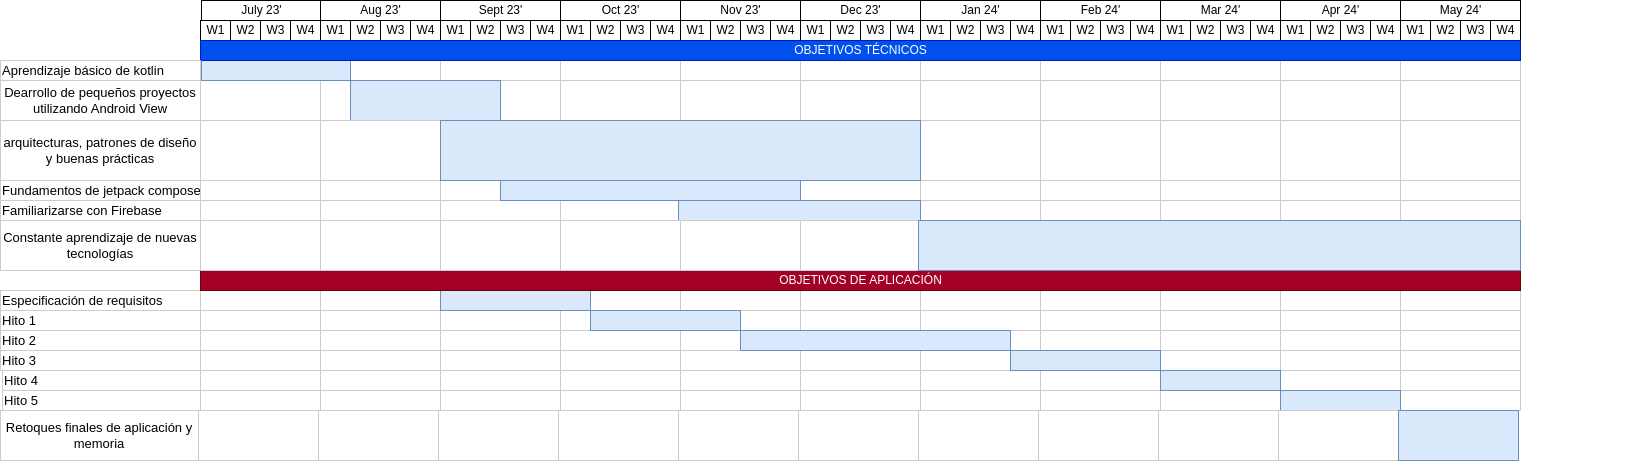
\includegraphics[width = 1\textwidth]{Imagenes/Bitmap/Gantt_Diagram.png}
	\caption{Diagrama de Gantt del proyecto}
	\label{fig:Gantt}
\end{figure}

Respecto a los hitos del proyecto, a continuación se muestra una lista con los casos de uso a desarrollar en cada hito:
\begin{itemize}
	\item Hito 1
	\begin{itemize}
		\item Registro/Baja de usuario.
		\item Modificar datos usuario.
		\item Login/Logout de usuario.
		\item Configurar app.
	\end{itemize}
	\item Hito 2
	\begin{itemize}
		\item Cambiar estado de profesional.
		\item Dar de alta/baja servicio.
		\item Modificar servicio.
		\item Listar servicios dados de alta.
		\item Añadir/Eliminar/Modificar categorías de servicios ofrecidos.
	\end{itemize}
	\item Hito 3
	\begin{itemize}
		\item Buscar servicio.
		\item Configurar búsqueda.
		\item Consultar profesional.
		\item Consultar cliente.
		\item Añadir/Quitar Profesional de lista de favoritos.
		\item Añadir/Modificar/Quitar cliente de lista de favoritos.
		\item Ver lista de favoritos.
	\end{itemize}
	\item Hito 4
	\begin{itemize}
		\item Contratar servicio.
		\item Chatear con profesional/cliente.
		\item Valorar cliente/profesional.
		\item Contestar solicitud de contratación.
	\end{itemize}
	\item Hito 5
	\begin{itemize}
		\item Consultar datos/estadísticas de profesional/clientes.
		\item Buscar clientes/profesionales.
		\item Modificar datos de clientes/profesionales/servicios ofrecidos.
		\item Dar de baja usuarios.
	\end{itemize}
\end{itemize}
Debido a que los casos de uso eran una aproximación inicial, según ha ido avanzando el proceso de desarrollo, algunos se han implementado antes, después, o se han descartado por no encajar bien en la aplicación. A pesar de esto, la planificación inicial, ha sido de gran utilidad como guía y ha servido para marcar correctamente los plazos de entrega, asimilando el proceso a como sería en un entorno real.
\chapter{Estado de la Cuestión}
\label{cap:estadoDeLaCuestion}

\section{Uber}
\begin{figure}[h]
	\centering
	
\includegraphics[width = 0.4\textwidth]{Imagenes/Fuentes/logo_Uber.png}
	\caption{Logotipo Uber}
	\label{fig:uber_logo}
\end{figure}
Uber \footnote{\url{https://www.uber.com}} es una aplicación muy conocida que sirve para contratar servicios de desplazamiento en V.T.C. (Vehículo de Transporte con Conductor), el motivo por el que se considera una aplicación relacionada con Profinder es que los servicios se contratan por proximidad, se utiliza la ubicación del usuario -al igual que se hace en Profinder- para encontrar los conductores más próximos, reduciendo así tiempos de espera y costes de desplazamiento innecesario. Uber se ha utilizado como una de las aplicaciones de referencia ya que representa muy bien el concepto que se ha buscado desde el principio con Profinder.

\section{Habitissimo}
\begin{figure}[h]
	\centering
	
\includegraphics[width = 0.4\textwidth]{Imagenes/Fuentes/habitissimo_logo.jpg}
	\caption{Logotipo Habitissimo}
	\label{fig:habitissimo_logo}
\end{figure}
Habitissimo \footnote{\url{https://www.habitissimo.es/}} es la posible competencia más directa que se ha encontrado. Es una aplicación en la que distintos profesionales pueden publicar ofertas de servicios, que los usuarios pueden contratar pidiendo un presupuesto. Esta aplicación está más enfocada a profesiones artesanales (carpintería, pintura, albañilería...) a diferencia de Profinder, que no está enfocada a ningún sector particular, sino que cuenta con distintas categorías que pueden ir ampliándose y ajustándose con el tiempo. Profinder también busca diferenciarse por tener un proceso más ágil que no dependa de ningún tipo de tercero y en el que se pueda tener un contacto más directo entre usuarios y profesionales. 

\section{Upwork}
\begin{figure}[h]
	\centering
	
\includegraphics[width = 0.4\textwidth]{Imagenes/Fuentes/logo_upwork.png}
	\caption{Logotipo Upwork}
	\label{fig:upwork_logo}
\end{figure}


\section{Booksy}
\begin{figure}[h]
	\centering
	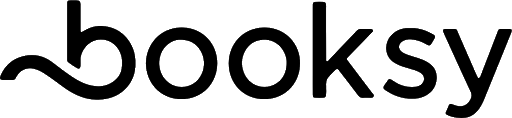
\includegraphics[width = 0.4\textwidth]{Imagenes/Fuentes/logo_booksy.png}
	\caption{Logotipo Booksy}
	\label{fig:booksy_logo}
\end{figure}
% \chapter{Descripción del Trabajo}
\label{cap:descripcionTrabajo}

Aquí comienza la descripción del trabajo realizado. Se deben incluir tantos capítulos como sea necesario para describir de la manera más completa posible el trabajo que se ha llevado a cabo. Como muestra la figura, está todo por hacer.

\section{Tecnlogías empleadas}
\section{Justificación del diseño y consideraciones técnicas fundamentales}
\section{Modelo de datos}
\include{Capitulos/tecnologiasEmpleadas}
\chapter{Arquitectura y modelo de datos}
\label{cap:modeloDeDatos}
En este capítulo se explicará la arquitectura y el modelo de datos utilizado en la aplicación. 

En la primera sección se explicará la arqitectura seguida en el proyecto, así como los patrones utilizados. Por otro lado, en la sección de modelo de datos, se hará una descripición de todas las estructuras de datos utilizadas, explicándolas brevemente para dar un poco de contexto, sin embargo, siempre se recomienda ver y tocar el código para entenderlo en profundidad. En segundo lugar se explicarán todos los servicios utilizados para mantener la persistencia: Firebase (principal herramienta utilizada como \textit{backend}), Datastore (se ha utilizado para guardar en local preferencias del sistema) y por último se explicará como se ha utilizado el patrón Singleton para evitar tener que usar una base de datos local como 
Room\hyperlink{cap:biblio}{\endnote{\textbf{Room}: \url{https://developer.android.com/training/data-storage/room/}}}, logrando así una aplicación completa.
\section{Arquitectura y patrones}
\subsection{CLEAN architecture}
\label{subsec:cleanArch}
La arquitectura CLEAN, originaria del libro \textit{Clean Architecture} (Martin, 2017)\hyperlink{cap:biblio}{\endnote{
\textit{Clean Architecture: A Craftsman's Guide to Software Structure and Design}, Robert C. Martin, 2017}}, es una forma de estructurar el software, dividiendolo en distintas capas que abstraigan el código y separen responsabilidades. Gracias al uso de esta arquitectura, se ha podido crear un proyecto escalable y robusto. También se han ahorrado muchos dolores de cabeza en los distintos procesos de refactorización ya que al haber tenido una estructura ordenada y bien definida, se han evitado posibles efectos secundarios por causa de los distintos cambios.

En Profinder se ha adaptado esta arquitectura a la programación en Android, dividiéndose así el código en cuatro capas explicadas a continuación:
\begin{enumerate}
    \item core: en esta capa van los recursos comunes que pueden ser accedidos por todas las demás capas, esta es una relación unidireccional ya que core no puede acceder a las demás capas. En este proyecto en particular se ha utilizado para guardar todo el boilerplate necesario para la aplicación del MVI (explicado en la apartado \ref{subsec:mvi}), modelos de datos para pruebas, y utilidades como la clase encargada de formatear las fechas y combinar los identificadores de usuarios.
    \item data: en esta capa es donde se gestionan todos los servicios y se preparan para ser enviados a la capa domain (explicada en el siguiente punto). Esta capa tiene toda la lógica de aplicación y es la encargada de decidir de dónde sacar los datos, todas las llamadas de red se hacen en esta capa. En muchos casos, esta capa tiene un modelo de datos propio (los datos tal cual llegan de los \textit{endpoints}) que adapta mediante el uso de \textit{mappers} para ser enviados a la siguiente capa.
    \item domain: En esta capa se encuentra la lógica de negocio de la aplicación, sería común a todas las versiones de la aplicación si se hicieran para otros sistemas operativos (IOS, Windows...) a excepción de la adecuación con el lenguaje de programación específico de cada sistema operativo, esto significa que no le ‘importa’ de donde vienen los datos, cuenta con una interfaz (denominada repositorio) en la que se ha definido el contrato con la capa de data y es ahí donde pide los datos que le deben llegar según su propio modelo (mapeados). Es en esta capa donde se definen los casos de uso, que actúan como contratos entre la capa de UI (explicada en el siguiente punto) y el repositorio. Esta implementación abstrae responsabilidades y ayuda a la encapsulación. 
    \item ui: Esta es toda la capa de interfaz de usuario de la aplicación, realizada utilizando \hyperlink{subsec:compose}{Jetpack compose} y siguiendo el patrón arquitectónico  MVI (\ref{subsec:mvi}). Las vistas como tal (denominadas \textit{Composables}) se comunican con los casos de uso (capa domain) a través de unas clases denominadas \textit{Viewmodels}\hyperlink{cap:biblio}{\endnote{\textbf{Viewmodels}: \url{https://developer.android.com/topic/libraries/architecture/viewmodel}}}.
\end{enumerate}

\hypertarget{subsec:mvi}{}
\subsection{MVI}
\label{subsec:mvi}
Debido a que en una aplicación móvil la mayor parte del trabajo se realiza en la interfaz de usuario, es habitual seguir patrones de diseño (mejor denominados: pseudo-arquitecturas). En el caso de Profinder había dos posibilidades: MVVM\hyperlink{cap:biblio}{\endnote{\textbf{MVVM}: \url{https://builtin.com/software-engineering-perspectives/mvvm-architecture}}} (Model-View-Viewmodel) o MVI (Model-View-Intent). Se decidió seguir el patrón MVI por ser más organizado y viable para aplicaciones de tamaño grande, a su vez es un patrón que se adapta muy bien al paradigma de programación en kotlin (programación funcional), su única desventaja es que introduce código de relleno para la estructuración (denominado boilerplate), pero esto a su vez ayuda a que sea más entendible por terceros a medida que aumenta el tamaño del proyecto. A continuación se explica en qué consiste esta pseudo-arquitectura y como se ha aplicado en el proyecto:
\begin{itemize}
    \item \textbf{Model}: es un término que puede variar en distintas pseudo-arquitecturas, en MVI es el que representa el estado de los datos, es inmutable y cuando se quiere cambiar algún atributo se destruye y se vuelve a crear con las nuevas modificaiones, esto ayuda a aumentar la testabilidad del código. Por ejemplo podemos tener un estado para la carga de datos (una  variable loading) y otro para el usuario (empieza siendo nulo y cuando se han cargado los datos se reescribe el estado con la nueva variable), en la figura \ref{fig:ejemplo_estado} se muestra el estado que se ha utilizado para el perfil de usuario.
    \begin{figure}[h]
        \centering
        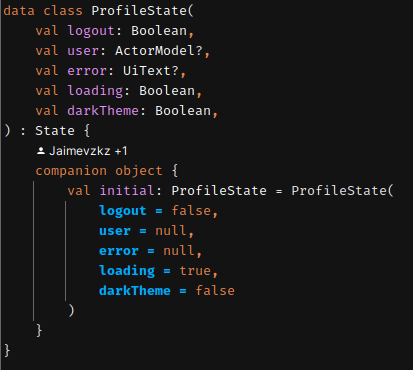
\includegraphics[width = 0.5\textwidth]{Imagenes/Fuentes/ejemplo_estado.png}
        \caption{Ejemplo de estado.}
        \label{fig:ejemplo_estado}
    \end{figure}
    \item \textbf{View}: se encarga de observar el estado y renderizar la vista de forma reactiva. Por ejemplo, en el caso de observar que cambia el valor de la variable loading, dibujaríamos un shimmer (pantalla de carga), cuando el valor de loading se pusiera a \textit{true} y tras comprobar que no hubiera errores, se dibujaría la vista como tal. Esto hace que la vista sea ‘tonta’ en el sentido de que no tiene que tomar ningún tipo de decisión, solo recibe unos datos en el estado y los pinta.
    \item \textbf{Intent}: se define como una acción (No confundir con la clase Intent de Android\hyperlink{cap:biblio}{\endnote{\textbf{Intent}: \url{https://developer.android.com/guide/components/}}}) que se lanza cuando el usuario realiza una acción (o el sistema solicita un cambio de estado). Estas acciones se procesan en un \textit{pipe} del viewmodel y van sobreescribiendo el estado. Es la forma que tiene la vista de cambiar los datos, cuando el usuario realiza una acción (como por ejemplo pulsar un botón), la vista lanza un \textit{intent} que se procesa, haciendo los cambios de estado necesarios, en la figura \ref{fig:ejemplo_intent} se muestran los \textit{intents} declarados para la vista de perfil de usuario.
    \begin{figure}[h]
        \centering
        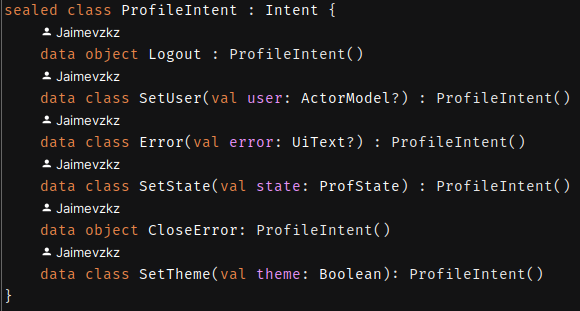
\includegraphics[width = 0.7\textwidth]{Imagenes/Fuentes/ejemplo_intent.png}
        \caption{Ejemplo de definición de los \textit{intents} de una vista.}
        \label{fig:ejemplo_intent}
    \end{figure}
\end{itemize}

Esta estructura define un flujo unidireccional de datos: La vista lanza intents que sobreescriben el estado, como consecuencia de este cambio de estado cambia la vista. Este flujo tiene muchas ventajas que ayudan a crear un código entendible, organizado y escalable. En la figura \ref{fig:visualMvi} se muestra de forma gráfica el ciclo
\hyperlink{cap:biblio}{\endnote{Imagen sacada del articulo publicado por Roberto Fuentes en \textit{Medium}: \href{https://medium.com/@robercoding/qué-es-y-cómo-funciona-la-arquitectura-mvi-desarrollo-android-kotlin-e6a161e1b2db}{\textbf{Fuentes on Medium}}}}.
\begin{figure}[h]
    \centering
    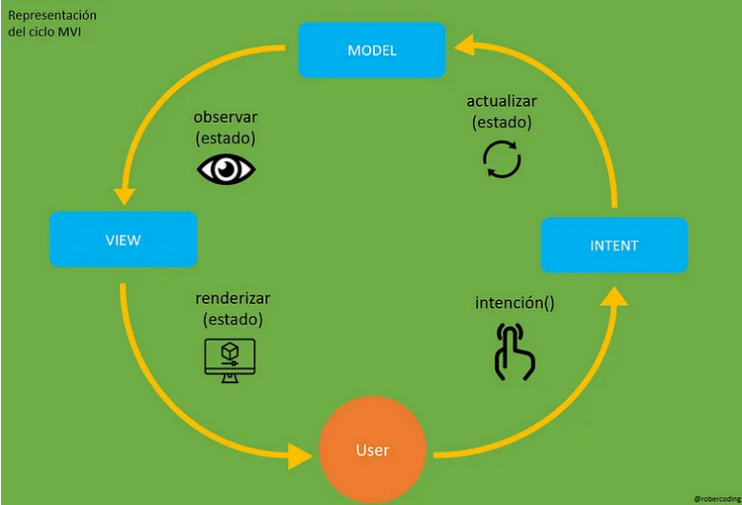
\includegraphics[width = 0.6\textwidth]{Imagenes/Fuentes/visual_mvi.png}
    \caption{Representación gráfica del ciclo MVI.}
    \label{fig:visualMvi}
\end{figure}

\subsection{Principios SOLID}
\label{subsec:solid}
Los principios SOLID son un conjunto de cinco principios de diseño de software que fueron introducidos en el libro \textit{Clean Code} (Martin, 2008)\hyperlink{cap:biblio}{\endnote{\textit{Clean Code: A Handbook of Agile Software Craftsmanship}, Robert C. Martin, 2008}}. Están destinados a guiar a los desarrolladores hacia la creación de código fuente limpio, modular, mantenible y extensible. A continuación se ha descrito brevemente cada uno de ellos, adjuntando una captura del código de la aplicación que lo implementa o una explicación de en qué parte del código se ha implementado cuando lo anterior no sea posible:
\begin{enumerate}
    \item Principio de Responsabilidad Única (\textit{Single Responsibility Principle}): establece que una clase debería tener una única razón para cambiar. En otras palabras, una clase debe tener una sola responsabilidad o función dentro del sistema. En la figura de ejemplo \ref{fig:change_state} se muestra como cualquier clase que implemente la interfaz tendrá la responsabilidad única de implementar el metodo \textit{invoke}.
    \begin{figure}[h]
        \centering
        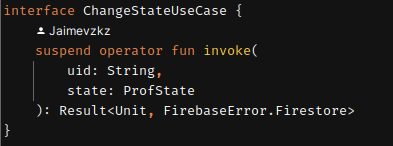
\includegraphics[width = 0.7\textwidth]{Imagenes/Fuentes/change_state.png}
        \caption{Ejemplo de primer principio SOLID.}
        \label{fig:change_state}
    \end{figure}
    \item Principio Abierto/Cerrado (\textit{Open/Closed Principle}): sostiene que las entidades de software (clases, módulos, funciones, etc.) deberían estar abiertas para su extensión pero cerradas para su modificación.
    
    Este principio se podría ver implementado por ejemplo en la funcionalidad \textit{profile}, en la que se podría añadir todo el código que se deseara para añadir funcionalidad sin tener que cambiar nada de lo ya implementado.
    \item Principio de Sustitución de Liskov (\textit{Liskov Substitution Principle}): establece que los objetos de un programa deben ser reemplazables por instancias de sus subtipos sin afectar la integridad del programa.
    
    En Profinder, este principio ha sido implementado por ejemplo en los \textit{viewmodels}, que heredan de la clase \textit{Baseviewmodel}. Cualquier instancia del objeto \textit{Baseviemodel} podría ser sustituido por la implementación de alguna de sus clases hijas sin que cambiara el comportamiento del programa.
    \item Principio de Segregación de la Interfaz (\textit{Interface Segregation Principle}):  sostiene que es mejor el uso de muchas interfaces pequeñas y concretas, mejor que una monolítica para evitar dependencias innecesarias.
    
    Esto se aplica en los casos de uso, cada caso de uso tiene una interfaz específica y concreta.
    \item Principio de Inversión de Dependencias (\textit{Dependency Inversion Principle}): establece que los módulos de alto nivel no deben depender (ni al revés) de los módulos de bajo nivel, ambos deben depender de abstracciones.
    
    Esto se cumple por ejemplo, como se muestra en la figura \ref{fig:ejemplo_reduce}, en la implementación \textit{reduce} de los viewmodel, esta función no tiene ninguna dependecia específica, sino que se adapta a cada caso recibiendo tipos genéricos.
    \begin{figure}[h]
        \centering
        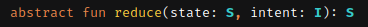
\includegraphics[width = 0.5\textwidth]{Imagenes/Fuentes/ejemplo_reduce.png}
        \caption{Ejemplo del quinto principio SOLID.}
        \label{fig:ejemplo_reduce}
    \end{figure}
\end{enumerate}

\section{Modelo de datos}
\label{sec:modeloDatos}
En esta sección se explica todo el modelo de datos y persistencia de la aplicación, en la figura \ref{fig:er_inicial} se puede encontrar un diagrama entidad relación abstracto que se hizo al comienzo del proyecto -cuando todavía no se sabía ni siquiera que tipo de base de datos se utilizaría- como modelo a seguir, algunos aspectos se han materializado de forma diferente en el modelo final (como por ejemplo la fusión de la estructuras de usuario y profesional o de las estructuras job y request) pero la esencia inicial se ha mantenido y el diagrama ha cumplido correctamente su papel como guía.
\begin{figure}[h]
    \centering
    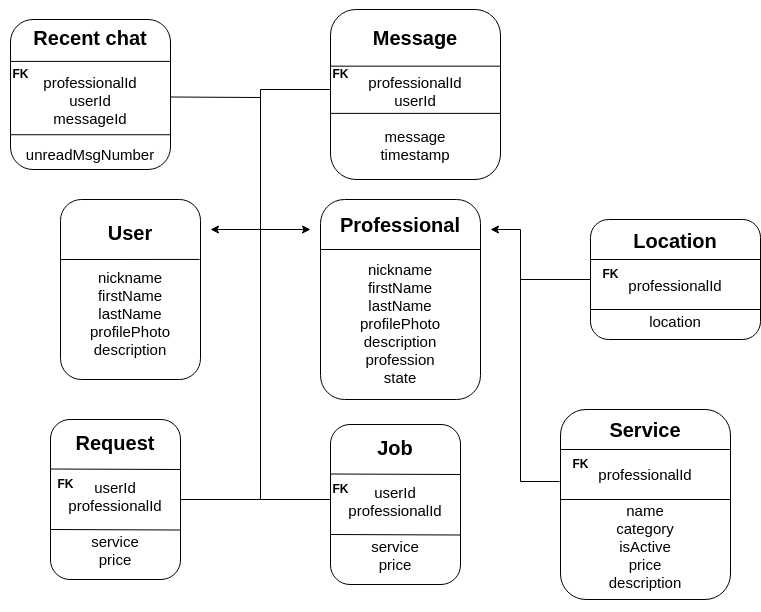
\includegraphics[width = 0.8\textwidth]{Imagenes/drawio/modelo_datos_inicial.png}
    \caption{Diagrama del modelo de datos inicial.}
    \label{fig:er_inicial}
\end{figure}
\subsection{Descripción detallada}
\begin{itemize}
    \item \textbf{ActorModel}: es la estructura de datos que almacena todos los datos de un actor, se usa la misma tanto para usuarios como para profesionales ya que admite campos nulos para aquellos atributos que solo corresponden a un tipo de actor, en esta estructura se guarda también el tipo de actor, la lista de favoritos (lista con otros \textit{ActorModel}), la calificación y el número de calificaciones tal y como se muestra en la figura \ref{fig:actorModel}.
    \begin{figure}[h]
        \centering
        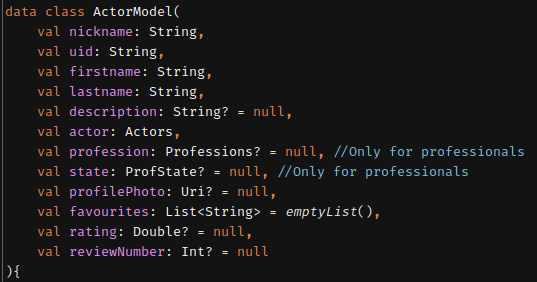
\includegraphics[width = 0.6\textwidth]{Imagenes/Fuentes/actorModel.png}
        \caption{Clase ActorModel.}
        \label{fig:actorModel}
    \end{figure}
    \item \textbf{ServiceModel}: guarda el modelo de un servicio, cuenta con distintos campos como la categoría del servicio, si está activo o no, y el propietario del servicio (un \textit{ActorModel}) tal y como se muestra en la figura \ref{fig:ServiceModel}.
    \begin{figure}[h]
        \centering
        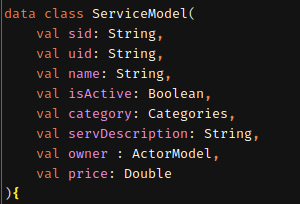
\includegraphics[width = 0.4\textwidth]{Imagenes/Fuentes/ServiceModel.png}
        \caption{Clase ServiceModel.}
        \label{fig:ServiceModel}
    \end{figure}
    \item \textbf{JobModel}: esta clase guarda tanto solicitudes de trabajo como trabajos activos, en un principio se hicieron dos clases separadas para esto, pero se comprobó que la funcionalidad era la misma y se unificó en una sola clase para evitar duplicaciones de código, relacionan el profesional, el usuario y el servicio tal y como se muestra en la figura \ref{fig:JobModel}.
    \begin{figure}[h]
        \centering
        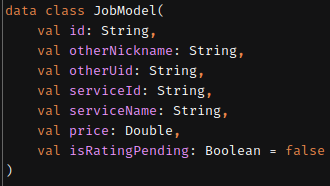
\includegraphics[width = 0.4\textwidth]{Imagenes/Fuentes/JobModel.png}
        \caption{Clase JobModel.}
        \label{fig:JobModel}
    \end{figure}
    \item \textbf{ChatListItemModel}: representa un item en la lista de chats recientes, guarda solo los campos necesarios para mostrar al usuario sin tener que volver a acceder a base de datos para sacar el \textit{ActorModel} completo, tal y como se muestra en la figura \ref{fig:ChatListItemModel}.
    \begin{figure}[h]
        \centering
        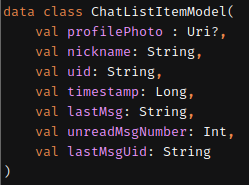
\includegraphics[width = 0.3\textwidth]{Imagenes/Fuentes/ChatListItemModel.png}
        \caption{Clase ChatListItemModel.}
        \label{fig:ChatListItemModel}
    \end{figure}
    \item \textbf{ChatMsgModel}: esta clase representa un mensaje en el chat, guarda el contenido del mensaje, un \textit{timestamp} para saber el momento exacto en el que se envió de cara a ordenarlo en la lista de mensajes, así como para mostrarle la hora al usuario y si el usuario es propietario (lo ha enviado él) o no (lo ha recibido) del mensaje, tal y como se muestra en la figura \ref{fig:ChatMsgModel}.
    \begin{figure}[h]
        \centering
        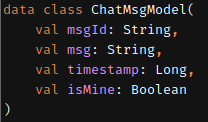
\includegraphics[width = 0.4\textwidth]{Imagenes/Fuentes/ChatMsgModel.png}
        \caption{Clase ChatMsgModel.}
        \label{fig:ChatMsgModel}
    \end{figure}
    \item \textbf{LocationModel}: representa la localización de un usuario, solo guarda los campos que es necesario mostrar en el mapa, la localización y el id del usuario (para poder extraer sus datos si fuera necesario) tal y como se muestra en la figura \ref{fig:LocationModel}.
    \begin{figure}[h]
        \centering
        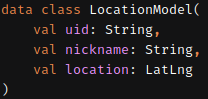
\includegraphics[width = 0.4\textwidth]{Imagenes/Fuentes/LocationModel.png}
        \caption{Clase LocationModel.}
        \label{fig:LocationModel}
    \end{figure}
    \item \textbf{Enums}: También se han usado una serie de enumerados para guardar cosas como los tipos de actores, las categorías de servicios, profesiones, etc. Esto hace que sea muy sencillo añadir nuevos en caso de necesidad sin tener que cambiar código existente, solo añadir nuevo (\textit{Open/Closed Principle}, véase el apartado \ref{subsec:solid}). En la figura \ref{fig:ejemplo_enum} se muestra un ejemplo del enumerado con los tipos de actores.
    
    \begin{figure}[h]
        \centering
        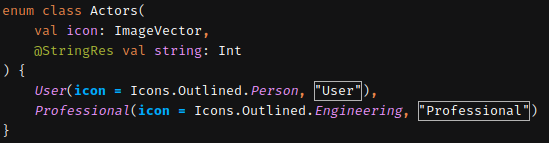
\includegraphics[width = 0.6\textwidth]{Imagenes/Fuentes/ejemplo_enum.png}
        \caption{Ejemplo de enumerado (actores).}
        \label{fig:ejemplo_enum}
    \end{figure}
\end{itemize}

\hypertarget{subsec:firebase}{}
\subsection{Firebase} 
\label{subsec:firebase}
Firebase \hyperlink{cap:biblio}{\endnote{\textbf{Firebase}: \url{https://firebase.google.com/}}} es una plataforma web desarrollada por Google que ofrece una amplia gama de servicios para ayudar a los desarrolladores a crear y mejorar aplicaciones. En Profinder, se ha utilizado como \textit{backend} para toda la aplicación y ha aportado la capacidad de plasmar el modelo de datos de la aplicación a una base datos, así como autenticación y almacenamiento para fotos. A continuación se ha explicado cada servicio utilizado.
\subsubsection{Authentication}
\label{subsec:firebaseAuth}
Firebase Authentication\hyperlink{cap:biblio}{\endnote{\textbf{Firebase Authentication}: \url{https://firebase.google.com/docs/auth/}}} es un servicio de autenticación que ahorra todo el proceso de gurdado y cifrado de contraseñas, también gestiona las sesiones de cada usuario, permitiendo mantener la sesión iniciada.Tiene compatibilidad para configurar diversos métodos de autenticación, sin embargo, en esta aplicación solo se ha considerado oportuno implementar la autenticación con \textit{email} y contraseña aunque si se quisiera sería sencillo añadir otros métodos. En la figura \ref{fig:ejemplo_auth} se muestra el panel de control de usuarios en el que se puede realizar un control sobre los mismos (como cambiar contraseñas o suspender cuentas).
\begin{figure}[h]
    \centering
    
\includegraphics[width = 1\textwidth]{Imagenes/Fuentes/ejemplo_auth.png}
    \caption{Captura de pantalla del panel de control de Firebase Authentication.}
    \label{fig:ejemplo_auth}
\end{figure}
\hypertarget{subsec:firestore}{}
\subsubsection{Firestore} 
Firebase Firestore \hyperlink{cap:biblio}{\endnote{\textbf{Firebase Firestore}: \url{https://firebase.google.com/docs/firestore/}}} ha sido la principal base de datos del proyecto, es de tipo no SQL lo cual ha presentado algunas ventajas pero también muchos desafios ya que en este tipo de bases de datos es muy fácil caer en la duplicación de datos y ha sido necesario gastar mucho tiempo en pensar la mejor forma de implementarla. 

En la figura \ref{fig:ejemplo_firestore} se muestra el panel de control de firestore donde se pueden ver, añadir y modificar datos de forma manual. 

La base de datos ha sido dividida en tres colecciones explicadas a continuación (véase el apéndice \ref{Appendix:bd_design} con el diagrama del diseño):
\begin{itemize}
    \item \textbf{users}: cada documento de esta colección se guarda con un id generado automáticamente y es donde se almacenan los datos de cada usuario, así como los \textit{jobs} y \textit{requests}.
    \item \textbf{services}: cada documento de esta colección se guarda con un id generado automáticamente y es donde se almacenan los datos de cada servicio.
    \item \textbf{locations}: cada elemento de esta colección representa la localización de un usuario, se generan con un id igual al id del usuario y guardan el \textit{nickname} a parte de la localización
\end{itemize}
\begin{figure}[h]
    \centering
    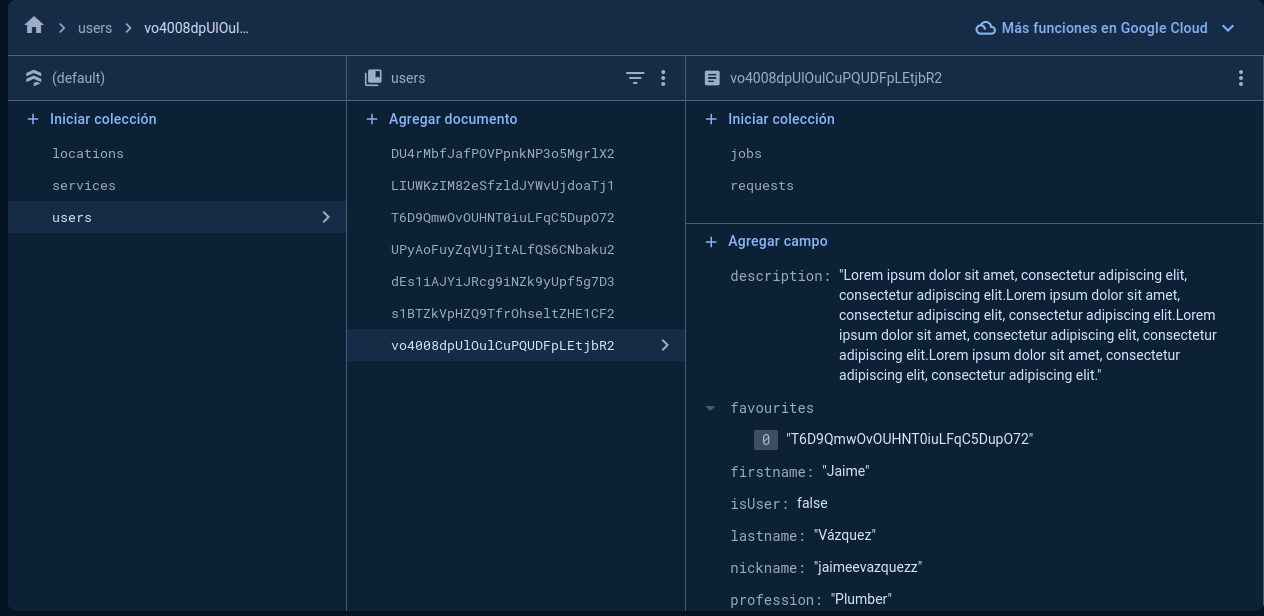
\includegraphics[width = 0.7\textwidth]{Imagenes/Fuentes/ejemplo_firestore.png}
    \caption{Captura de pantalla del panel de control de la base de datos Firestore.}
    \label{fig:ejemplo_firestore}
\end{figure}
\hypertarget{subsec:realtime}{}
\subsubsection{Realtime Database}
Realtime database\hyperlink{cap:biblio}{\endnote{\textbf{Realtime database}: \url{https://firebase.google.com/docs/database/}}} es una base datos de baja latencia, menos sofisticada que \hyperlink{subsec:firestore}{Firestore} pero cuyas funcionalidades han encajado perfectamente con las necesidades del proyecto. Se ha utilizado para toda la funcionalidad de chat ya que al ser los mensajes en tiempo real, era necesario que la latencia fuera mínima. 

En Realtime, los datos se guardan en formato JSON (\textit{JavaScript Object Notation}). Su estructura se ha divido en la lista de chats recientes (conteniendo atributos como el último mensaje, los participantes, la hora y el número de mensajes sin leer por cada conversación entre dos actores de la aplicación) y los chats en sí (conteniendo cada mensaje de una conversación con la hora en que fue mandado). En la figura \ref{fig:ejemplo_realtime} se muestra el panel de control de realtime donde se pueden ver, añadir, eliminar y modificar datos, aunque es menos sofisticado que el panel de control de firestore.
\begin{figure}[h]
    \centering
    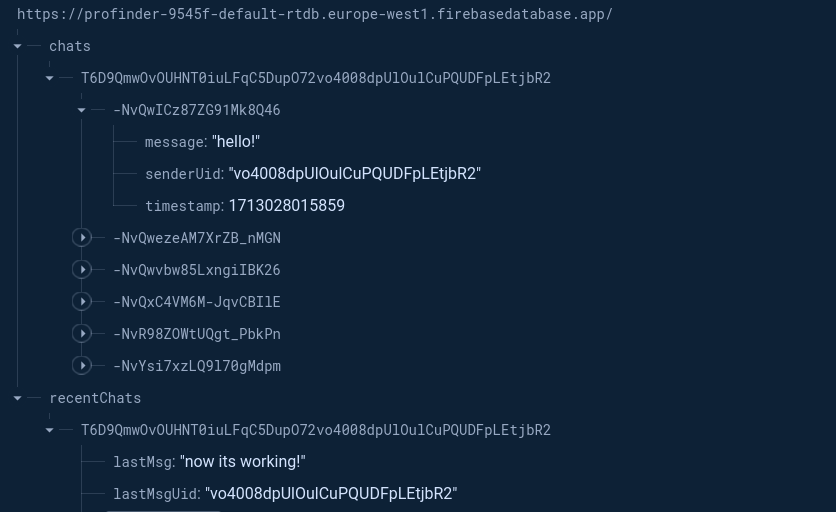
\includegraphics[width = 0.6\textwidth]{Imagenes/Fuentes/ejemplo_realtime.png}
    \caption{Captura de pantalla de la estructura de Realtime Database}
    \label{fig:ejemplo_realtime}
\end{figure}
\subsubsection{Storage}
Firebase storage\hyperlink{cap:biblio}{\endnote{\textbf{Firebase storage}: \url{https://firebase.google.com/docs/storage/}}} es un servicio de alamcenamiento en la nube. Se ha utilizado para almacenar las fotos de perfil de los actores de la aplicacion. Cada foto de perfil se guarda en una carpeta cuyo nombre es el id del actor y se accede a ella a traves de una uri autogenerada que se procesa en la aplicación usando \hyperlink{subsec:coil}{Coil}.

\hypertarget{subsec:datastore}{}
\subsection{Datastore}
Datastore\hyperlink{cap:biblio}{\endnote{\textbf{Datastore}: \url{https://developer.android.com/topic/libraries/architecture/datastore}}} es un sistema de almacenamiento persistente que permite guardar pares clave valor en la aplicación para un acceso rápido a través de 
corrutinas\hyperlink{cap:biblio}{\endnote{\textbf{Corrutinas}: \url{https://developer.android.com/kotlin/coroutines}}} En el caso de Profinder se ha utilizado para guardar 2 cosas:
\begin{itemize}
    \item \textbf{Tema de la aplicación}: de tal forma que cuando se cambia su valor, devuelve un flow\hyperlink{cap:biblio}{\endnote{\textbf{Flows}: \url{https://developer.android.com/kotlin/flow}}} que indica a la Main Activity el tema que debe utilizar. Este tema se mantiene en caché por lo que se podría cerrar la aplicación y al abrirla se recordaría el tema establecido.
    \item \textbf{El id del usuario iniciado}: De tal forma que cuando se necesiten datos del usuario desde cualquier parte de la app se puede conseguir el id (que es único en base de datos) según necesidad, esto servirá para un acceso más rápido en Firestore debido a que es una base de datos que se indexa por este campo.
\end{itemize}

\subsection{Uso del patrón Singleton como modelo de persistencia}
\label{subsec:singletonComoModelo}
En la programación Android, la persistencia de datos es muy importante ya que al contrario que en otro tipo de programas, cada poco tiempo se borran todos los datos no persistidos para evitar que la aplicación ocupe demasiado espacio en el dispositivo. En este contexto es donde se presenta el problema.

A lo largo del desarrollo de otras aplicaciones (en preparación a esta) se encontró que el uso de una base de datos local suponía una carga de espacio en la aplicación y en tiempo de compilación que la ralentizaba, más allá de esto, las necesidades de Profinder implicaban que los datos fueran actualizados cada no demasiado tiempo puesto que tanto servicios; como favoritos; como los datos de usuario están diseñados para cambiar con frecuencia entre los distintos actores de la aplicación. Por estos motivos se decidió buscar un sistema alternativo que se adecuara a las necesidades de la aplicación: actualización frecuente y poca carga en memoria sin tener que estar accediendo constantemente al servicio remoto (\hyperlink{subsec:firestore}{Firestore}) ya que esto supondría un coste económico.

Esta solución se ha implementado siguiendo el patrón \textit{Singleton}. Los datos a persistir se almacenan en una clase que los guarda de la siguiente forma: si los datos están cacheados los devuelve, si no, los saca del servicio remoto, los cachea y los devuelve. De esta forma la próxima vez que se accedan los datos, estarán cacheados y no hará falta llamar al servicio remoto. La figura \ref{fig:ejemplo_singleton1} muestra la función que implementa la lógica descrita.

\begin{figure}[h]
    \centering
    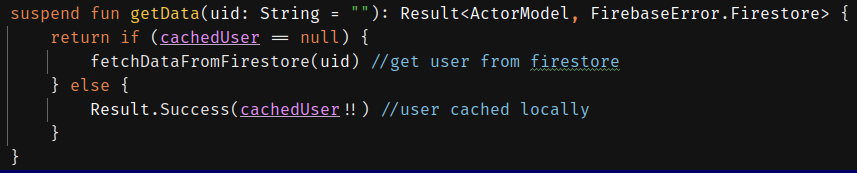
\includegraphics[width = 0.9\textwidth]{Imagenes/Fuentes/ejemplo_singleton1.png}
    \caption{Ejemplo de función getData()}
    \label{fig:ejemplo_singleton1}
\end{figure}

Para acceder a esta función es donde creamos el Singleton (figura \ref{fig:ejemplo_singleton2}) que será accedido desde cualquier lugar donde se necesiten los datos.
\begin{figure}[h]
    \centering
    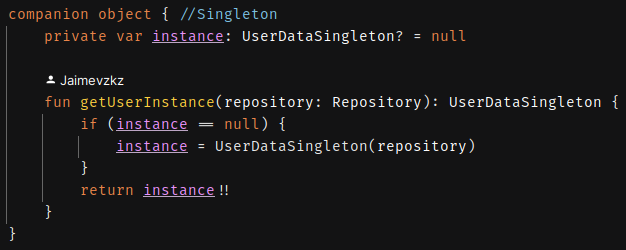
\includegraphics[width = 0.9\textwidth]{Imagenes/Fuentes/ejemplo_singleton2.png}
    \caption{Ejemplo de Singleton con datos de usuario}
    \label{fig:ejemplo_singleton2}
\end{figure}
\chapter{Diseño e implementación}
\label{cap:disenoEImpl}
En este capítulo, se explican todos los conceptos y decisiones que se han considerado relevantes para el diseño de la aplicación, así como el proceso de implementación, dividiendo la aplicación por bloques funcionales.

\section{Diseño}
El objetivo en lo relativo al diseño, ha sido crear una aplicación escalable a distintos idiomas, con una experiencia de usuario agradable, bonita a la vista y que se ajuste a los principios \textit{open source}. A continuación, se explica en detalle como se han intentado lograr estos objetivos.

\subsection{Experiencia de usuario}
Para conseguir una buena experiencia de usuario, se han intentado seguir una serie de principios de diseño para aplicaciones. Asimismo, se ha intentado mantener una paleta de colores homogénea en la aplicación, usando material design (véase el apartado \ref{subsec:material_design}) y  unas interfaces de usuario minimalistas, a la vez que autoexplicativas. A continuación se explican algunas de las medidas que se han tomado, para lograr los objetivos anteriores.
\begin{itemize}
    \item Para la nevegación a través de la aplicación, se ha utilizado una \textit{bottom bar} (como se ve en la figura \ref{fig:ejemplo_bottombar}), este es un elemento típico en aplicaciones, lo que implica que culaquier usuario, aunque no haya utilizado la aplicación nunca, sabrá navegar por ella.
    \begin{figure}[h]
        \centering
        
\includegraphics[width = 0.6\textwidth]{Imagenes/Fuentes/ejemplo_bottombar.png}
        \caption{Ejemplo de la bottom bar.}
        \label{fig:ejemplo_bottombar}
    \end{figure}
    \item La home, es la pantalla principal de la aplicación, por lo que navegar a ella no puede implicar tener más de una pantalla entre medias, esto quiere decir que, desde cualquier pantalla de la aplicación debe ser posible ir a la home sin pulsar más de dos botones. 
    \item Las decisiones importantes a tomar en la aplicación deben ser ‘más dificiles’, en el sentido de que deben implicar más pasos para evitar que el usuario las tome por accidente. Un ejemplo de esto, puede ser el cierre de sesión, ya que el botón se encuentra en la esquina superior izquierda, más difícil de alcanzar con los pulgares; Y al pulsarlo, se muestra un mensaje de confirmación. 
    \item Se ha trabajado en dar un buen feedback al usuario de las acciones realizadas en la aplicación, mostrando mensajes explicativos. También, se ha intentado que el usuario sepa en todo momento, lo que esta pasando, por ejemplo, mostrando pantallas de carga en los momentos de espera de datos. 
\end{itemize}

\subsection{Open source}
\label{subsec:openSource}
El código \textit{open source} (abierto, significando esto que el código desarrollado es público para cualquiera que lo quiera ver), es un movimiento socio-tecnólogico que comenzó en la decada de 1980, cuando Richard Stallman, considerado por muchos el padre del movimiento de \textit{open source} o \textit{free open source} (tomando la denotación de \textit{free} como libre no como gratuito),fundó la \textit{Free Software Foundation} (Fundación de código libre)\hyperlink{cap:biblio}{\endnote{\textbf{Free Software Foundation}: \url{https://www.fsf.org/}}}, así como el sitema operativo GNU\hyperlink{cap:biblio}{\endnote{\textbf{GNU}: \url{https://www.gnu.org/}}} (\textit{GNU's not Unix}). Richard, creía que el software debía ser  creado de forma colaborativa y libremente compartido. Otro gran exponente de este movimiento (aunque con distintas motivaciones), fue el finlandés Linus Torwalds, creador del kernel Linux (GNU-Linux es el sistema operativo con el que se está realizando esta memoria y todo el proceso de desarrollo).

En este contexto, se ha intentado desarrollar Profinder, siguiendo los principios \textit{open source} e intentando utilizar la mayor cantidad de herramientas de código abierto posible. Algunos ejemplos a parte de los que se han ido mencionando a lo largo de esta memoria, pueden ser Firefox\hyperlink{cap:biblio}{\endnote{\textbf{Firefox}: \url{https://www.mozilla.org/es-ES/firefox/}}}, Neovim\hyperlink{cap:biblio}{\endnote{\textbf{Neovim}: \url{https://neovim.io/}}} y Linux\hyperlink{cap:biblio}{\endnote{\textbf{Linux}: \url{https://www.linux.org/pages/}}}, entre otros. Asimismo, se ha decidido que todo el código de este proyecto sea libre (siendo posible revisarlo, distribuirlo y modificarlo), así como el proceso seguido para hacerlo.

La mayoría del contenido en este apartado ha tomado las referencias del libro \textit{The Innovators} (Isaacson, 2015)\hyperlink{cap:biblio}{\endnote{\textit{The Innovators: How a Group of Hackers, Geniuses and Geeks Created the Digital Revolution}, Walter Isaacson, 2015}}. 

\subsection{Idiomas}
Con el objetivo de hacer el proyecto lo mas ‘universal’ posible, el idioma principal utilizado para el desarrollo de Profinder (código, apuntes, \textit{commits}), ha sido el inglés. Sin embargo, todo los literales de texto que aparecen en la aplicación, han sido incluidos en un archivo (\textit{strings.xml}), en la figura \ref{fig:stringXml} se puede ver un ejemplo del mismo. El contenido de este fichero ha sido luego traducido al español, de tal forma que dependiendo del idioma del dispositivo del usuario, la aplicación estará en español o en inglés. Este mismo proceso podría ser llevado a cabo para añadir cualquier idioma.
\begin{figure}[h]
    \centering
    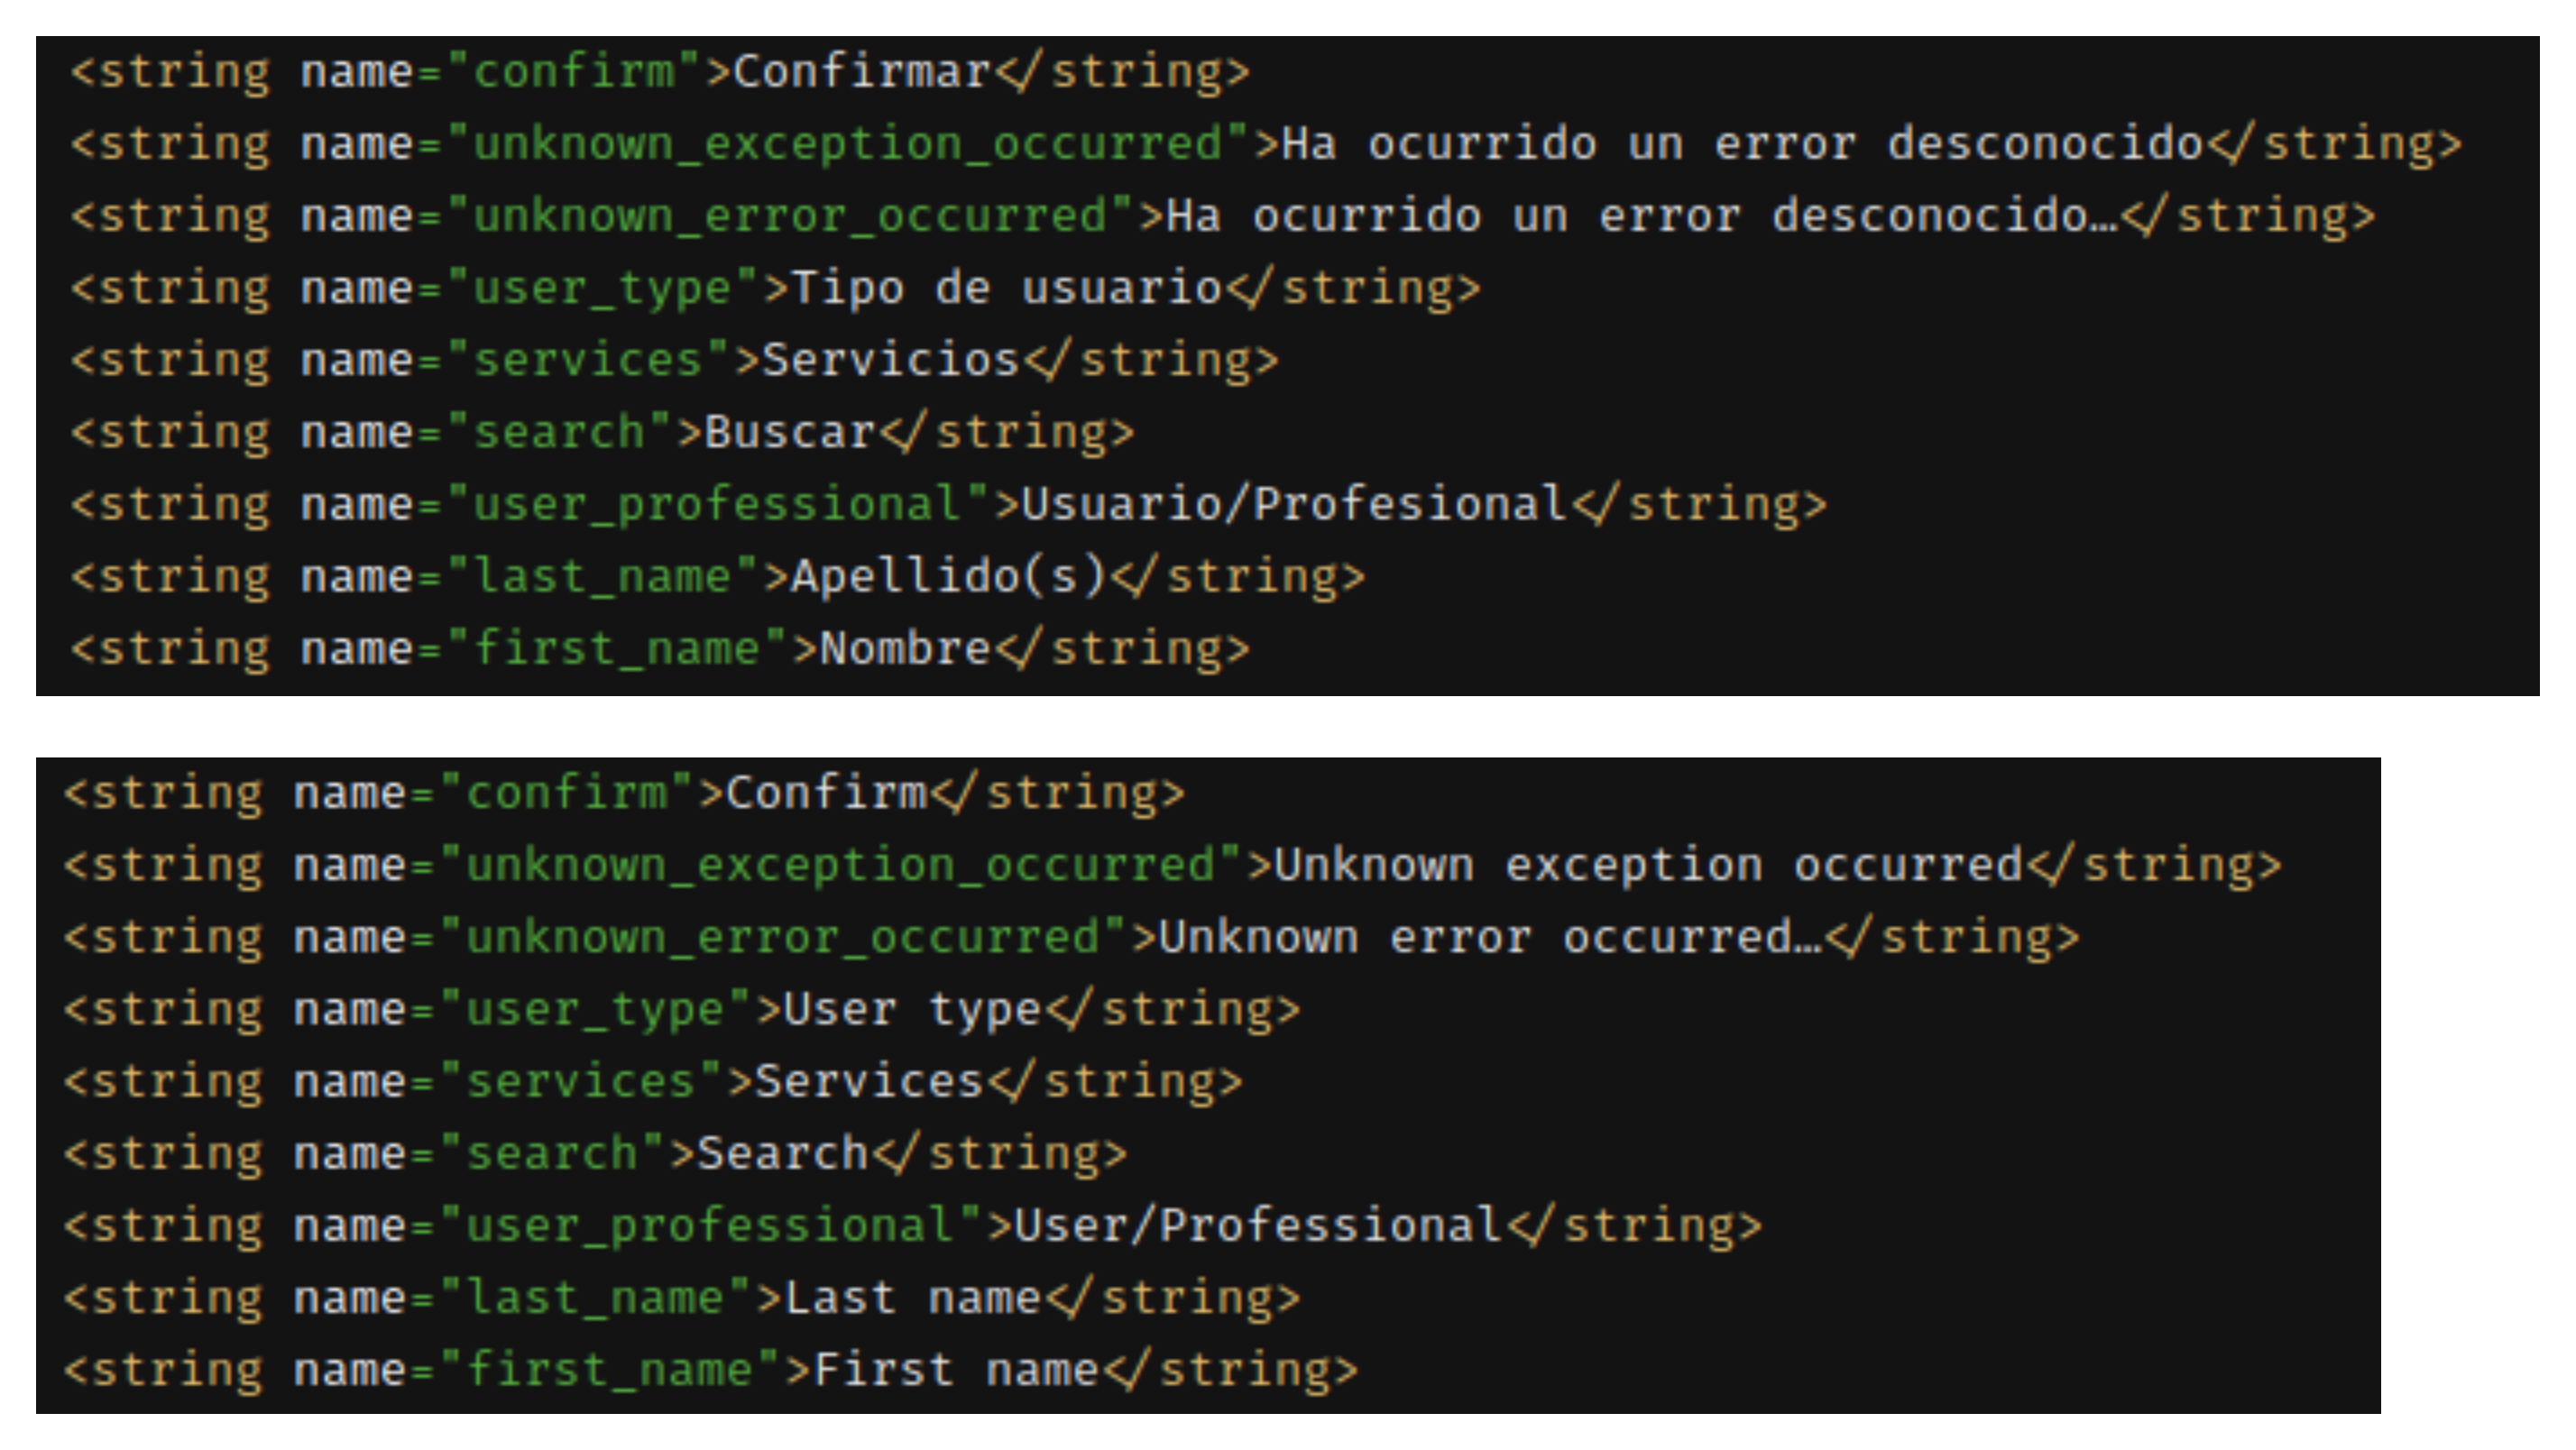
\includegraphics[width = 0.7\textwidth]{Imagenes/Fuentes/stringsXml.png}
    \caption{Parte del fichero strings.xml en su versión en inglés y español.}
    \label{fig:stringXml}
\end{figure}

\section{Implementación}
La implementación, se ha dividido en cinco grupos con funcionalidades relacionadas: autenticación, usuarios y profesionales, trabajos y servicio; Y chat. 

De cada grupo, se explicarán las consideraciones fundamentales que se han tenido en cuenta a nivel de código. También se explicará con detalle, el sistema de gestión de errores que ha sido utilizado por todos los bloques.
\subsection{Autenticación} 
Este bloque, incluye las funcionalidades de inicio de sesión, registro, cierre de sesión y mantenimiento de sesión iniciada. Todas estas implementaciones, han utilizado Firebase authentication (\ref{subsec:firebaseAuth}), como servicio de \textit{backend}.

El incio de sesión y el registro, han sido implementados usando formularios para los campos requeridos, para ello se han utilizado \textit{Textfields}, un componente que ofrece Compose para el \textit{input} de cadenas de texto. También, se ha comprobado que la cadena introducida por el usuario era correcta de forma dinámica (véase la figura \ref{fig:textfield}). 
\begin{figure}[h]
    \centering
    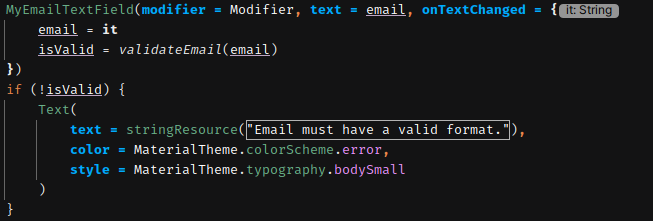
\includegraphics[width = 0.6\textwidth]{Imagenes/Fuentes/textfield.png}
    \caption{Ejemplo de validación del campo email.}
    \label{fig:textfield}
\end{figure}

El mantenimiento de la sesión, sirve para que el usuario no tenga que identificarse cada vez que abra la aplicación, sino que se guarden sus credenciales durante un tiempo determinado (en caso de cierre de sesión se eliminan). Para ello, se ha utilizado la \textit{Splash Screen}, de tal forma que al entrar en la aplicación, se comprueba si existe sesión; Si existe, se redirige al usuario a la \textit{home}; Sino, se le redirige a la pantalla de inicio de sesión (como se muestra en la figura \ref{fig:splashDest}). 
\begin{figure}[h]
    \centering
    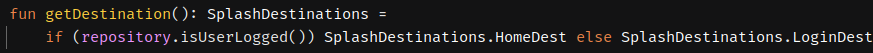
\includegraphics[width = 1\textwidth]{Imagenes/Fuentes/splashDest.png}
    \caption{Función que comprueba si hay una sesión guardada.}
    \label{fig:splashDest}
\end{figure}

\subsection{Usuarios y profesionales} 
Este bloque, incluye las funcionalidades de perfil, editar datos, vista de perfil, lista de favoritos y búsqueda.

En la pantalla de perfil, se ha implementado también la funcionalidad de cambio de tema de la aplicación. Se ha mantenido la persistencia de datos utilizando un \textit{Singleton} (ver el apartado \ref{subsec:singletonComoModelo}), gracias a esto, los datos se sacan de Firestore al iniciar sesión, y se mantienen un tiempo limitado, tras el cual se vuelven a sacar de base de datos, esto consigue una actualización frecuente (si por ejemplo, cambias los datos de la misma cuenta con otro dispositivo). Esta implementación, también ha sido utilizada para la lista de favoritos.

Para la función de ver el perfil de otro usuario, también se ha seguido este método pero con motivación distinta, el objetivo era evitar que si un usuario pulsaba el botón de ver un perfil, y al poco tiempo volvía a pulsar en el mismo perfil se llamara dos veces al servicio remoto. Lo que se ha conseguido, es que al pulsar para ver un perfil, este se cachee en el \textit{Singleton}, por si se realiza la misma acción. En cambio, si el siguiente perfil a ver es diferente, se vacía la cache y se llena con el nuevo perfil.

A la hora editar los datos del perfil, se ha tenido en cuenta la implementación de estos \textit{Singletons}, debido a que hay que asegurarse de que la copia en cache y en remoto se mantinenen sincronizadas. Esto supone, un pequeño esfuerzo extra, pero permite reducir el coste de llamadas remotas.

La búsqueda se ha implementado sacando el id, nombre completo, nombre de usuario, foto de perfil y tipo de actor de cada profesional. Cuando un item de la lista mostrada es pulsado, se saca la estructura de actor completa de base de datos usando el id de usuario y se muestra su perfil. 

\subsection{Trabajos y Servicios} 
Los trabajos se han dividido en 2 partes: solicitudes y trabajos. Se han guardado como dos listas distintas, para cada actor con los ids de los implicados, nombre de servicio, precio y nombre de usuario del otro actor. Su implementación a nivel de código ha sido igual, variando solo en el lugar donde mostrar cada lista. Esto ha ahorrado mucho código duplicado. Se ha utilizado un \textit{booleano}, como parámetro para diferenciar si se trata de una solicitud o un trabajo (ver figura \ref{fig:getJobOrRequest}).
\begin{figure}[h]
    \centering
    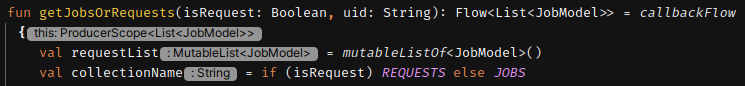
\includegraphics[width = 0.8\textwidth]{Imagenes/Fuentes/getJobOrRequest.png}
    \caption{Ejemplo de función condicionada por solicitud o trabajo.}
    \label{fig:getJobOrRequest}
\end{figure}

Por otro lado, los servicios que también se han implementado usando un \textit{Singleton} por las razones comentadas previamente, en la aplicación se utilizan como una lista de \textit{ServiceModel}, guardando el id del profesional al que pertenecen, para poder ser clasificados. La lista de servicios mostrada a los usuarios recoge todos los servicios activos de la aplicación debido a que por ahora el número no es demasiado grande, a pesar de esto, en el futuro se podrían filtrar y ordenar por otros atributos a parte del nombre, o mostrar una lista con un máximo número de elementos a la que se le podrían ir añadiendo más (cargándolos de base de datos), a medida que el usuario atraviesa la lista. Por otro lado, a los profesionales se les divide la pantalla de servicios, en activos e inactivos (dividiendo la lista de todos los servicios de un profesional sacados de base de datos en dos), a la hora de cambiar la actividad de un servicio también ha sido necesario cambiar el dato en local y remoto. Esto también se hace al eliminar servicios o añadir nuevos.

\subsection{Chat} 
La implementación del modulo de Chat, ha sido uno de los mayores desafíos de la aplicación a nivel lógico y de estructura de datos, debido a que en un comienzo, todos los modelos que se intentaron usar duplicaban muchos datos, haciendo la funcionalidad muy difícil de mantener. Al final se consiguió maximizar la eficiencia de las estructuras, dividiendo la funcionalidad en dos colecciones (en el aprtado \ref{sec:modeloDatos} se explica el modelo de datos en detalle). 

Otro gran problema al inicio, fue la necesidad de que todo se actualizara en tiempo real, para ello fue muy útil, aunque difícil a nivel programático, el uso de \textit{flows} (ver figura \ref{fig:flows_impl} como ejemplo de la implementación de flows), que en combinación con la capacidad reactiva de Jetpack Compose, hicieron posible una latencia mínima.
\begin{figure}[h]
    \centering
    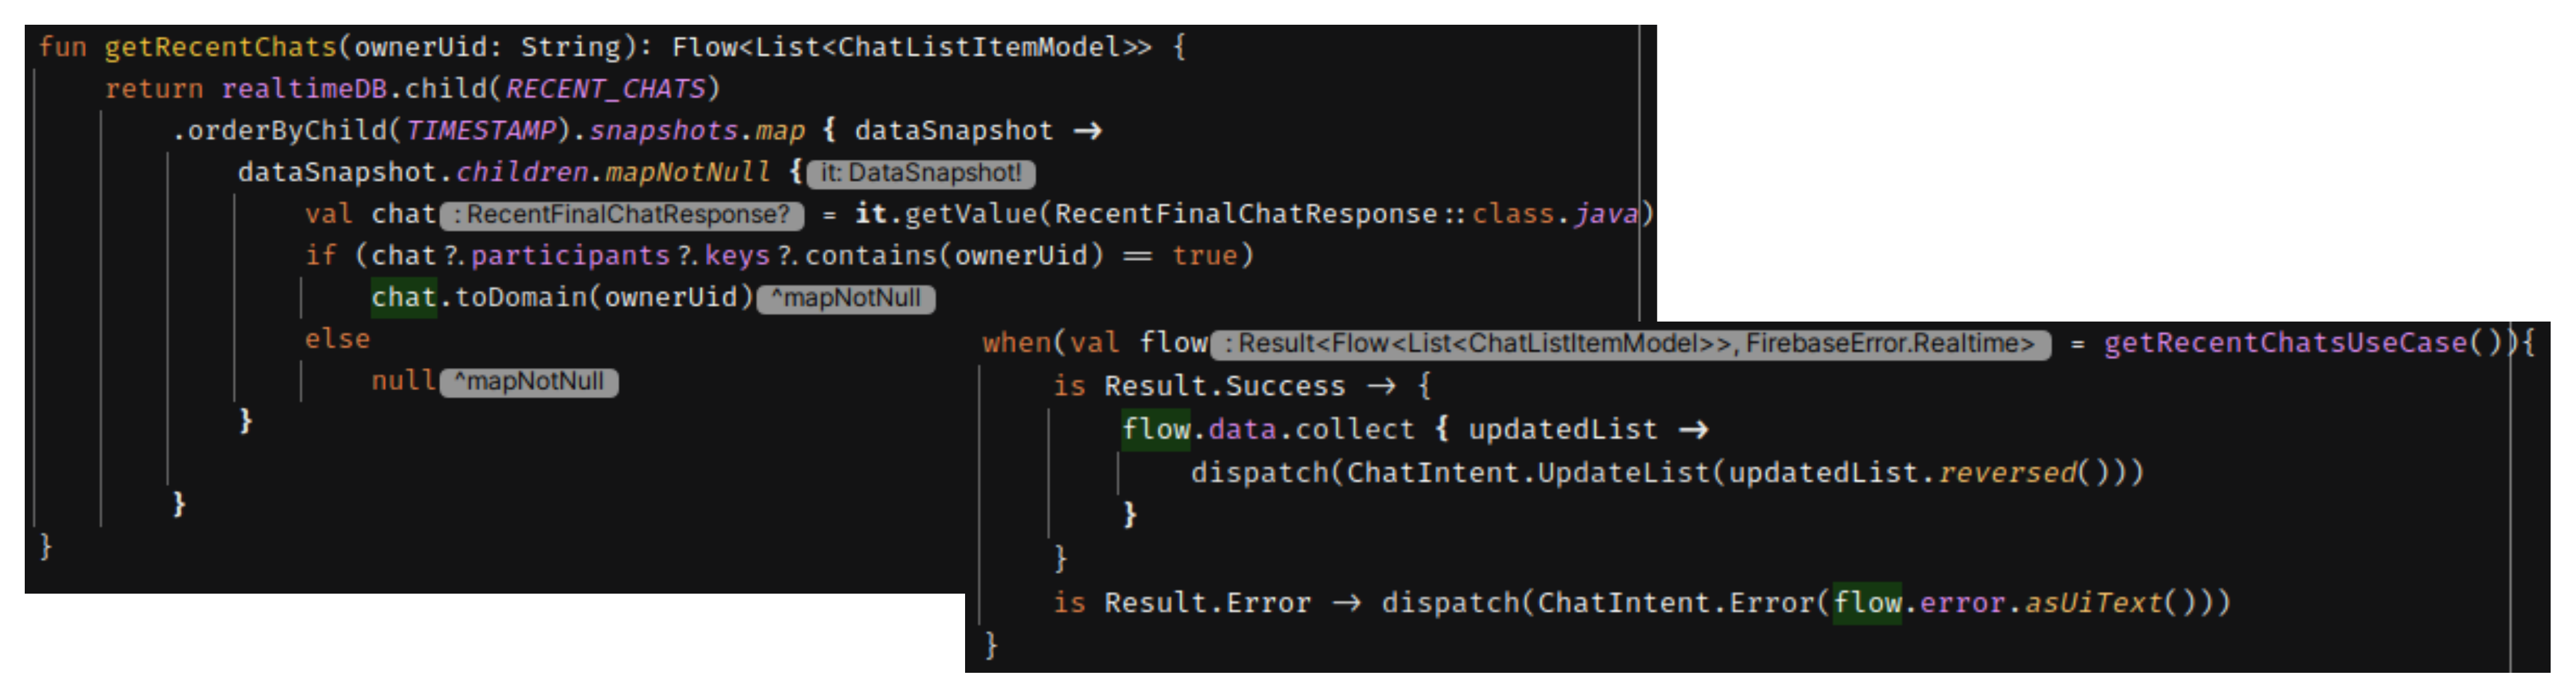
\includegraphics[width = 1\textwidth]{Imagenes/Fuentes/flows_impl2.png}
    \caption{Ejemplo de uso de flows para sacar los chats recientes y recogerlos en el viewmodel.}
    \label{fig:flows_impl}
\end{figure}

\subsection{Gestión de errores} 
Para conseguir una gestión de errores eficiente y generalizada, se han desarrollado una serie de clases, basadas en la estructura propuesta por el creador de contenido Philipp Lackner\hyperlink{cap:biblio}{\endnote{\textbf{Philipp Lackner on Error handling}: \url{https://www.youtube.com/watch?v=MiLN2vs2Oe0}}} y personalizadas según las necesidades específicas de la aplicación. Que en conjunto, sirven como sistema bien estructurado que proporciona una forma cómoda de gestionar errores, respetando todos los principios de arquitectura limpia, mencionados en el apartado \ref{subsec:cleanArch}. A continuación se explican todas las clases que se han creado, es posible que solo con la explicación que viene a continuación, no se entienda el sistema en su totalidad, pero el lector tendrá disponible el código fuente para verlo aplicado y si es necesario clonar el repositorio para probarlo haciendo cambios.

En primer lugar, se ha creado la interfaz \textit{Error}, mostrada en la figura \ref{fig:error_interface}, que servirá para identificar todos los tipos de errores declarados.
\begin{figure}[h]
    \centering
    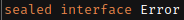
\includegraphics[width = 0.3\textwidth]{Imagenes/Fuentes/error_interface.png}
    \caption{Interfaz Error.}
    \label{fig:error_interface}
\end{figure}

En segundo, lugar se ha creado la interfaz Result (se ha llamado así a pesar de que ya haya una clase con este nombre en la biblioteca estandar por considerarse el más apropiado). Esta es la interfaz principal que utilizan todas las funciones de la aplicación que devuelvan datos. Tiene dos parametros genéricos, que cambiarán en cada caso específico -véase la figura \ref{fig:ejemplo_result}-, uno para los datos devueltos y otro para el tipo de error, también cuenta con los dos posibles resultados que puede devolver una función que implemente esta interfaz: 
\begin{itemize}
    \item \textbf{Success}: para el caso de éxito, llevará como parámetro los datos devueltos.
    \item \textbf{Error}: distinto de la interfaz explicada anteriormente, será lo que se devuelva en caso de error en la llamada a función y llevará como parámetro una clase que implemente la interfaz \textit{Error}.
\end{itemize}
\begin{figure}[h]
    \centering
    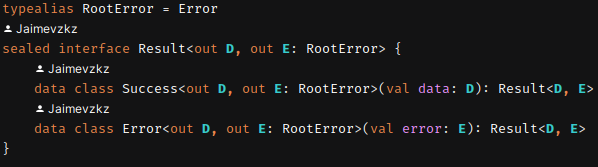
\includegraphics[width = 0.8\textwidth]{Imagenes/Fuentes/ejemplo_result.png}
    \caption{Interfaz Result.}
    \label{fig:ejemplo_result}
\end{figure}

Lo siguiente será crear tantas interfaces como sean necesarias, e implementen \textit{Error}. En Profinder, solo ha sido necesario crear una que englobara todos los errores relativos a \hyperlink{subsec:firebase}{Firebase}, sin embargo, es un sistema escalable a futuro.

Dentro de cada una de estas interfaces se declaran todos los tipos de errores (relativos a \hyperlink{subsec:firebase}{Firebase} por ejemplo, véase la figura \ref{fig:ejemplo_tipo_error}) como clases enumeradas, consiguiendo así, que cada uno sea un enumerado que se gestiona de forma independiente en las distintas capas de la aplicación.
\newpage
\begin{figure}[h]
    \centering
    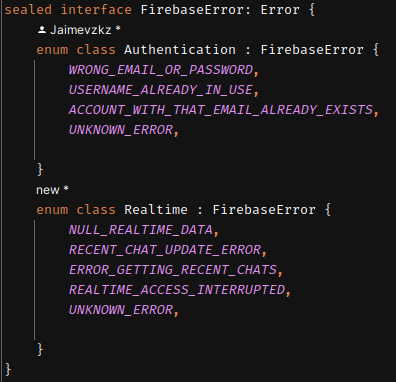
\includegraphics[width = 0.7\textwidth]{Imagenes/Fuentes/ejemplo_tipo_error.png}
    \caption{Ejemplo de tipo de error.}
    \label{fig:ejemplo_tipo_error}
\end{figure}

Con todo lo anterior, la gestión de errores se convierte en algo sencillo, las funciones deberán devolver un tipo \textit{Result} (figura \ref{fig:ejemplo_impl_result}).
\begin{figure}[h]
    \centering
    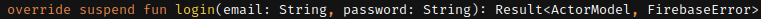
\includegraphics[width = 0.9\textwidth]{Imagenes/Fuentes/ejemplo_impl_result.png}
    \caption{Ejemplo de implementación de Result.}
    \label{fig:ejemplo_impl_result}
\end{figure}

Y en las llamadas a función se podrá gestionar si hay un error dividiendo los casos con una expresión
\textit{when}\hyperlink{cap:biblio}{\endnote{\textbf{when}: \url{https://www.programiz.com/kotlin-programming/when-expression}}}, como se ve en lafigura \ref{fig:llamada_funcion_result}.
\begin{figure}[h]
    \centering
    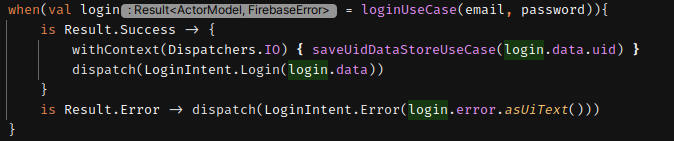
\includegraphics[width = 0.8\textwidth]{Imagenes/Fuentes/llamada_funcion_result.png}
    \caption{Ejemplo de llamada a función implementando Result.}
    \label{fig:llamada_funcion_result}
\end{figure}
\chapter{Conclusiones y Trabajo Futuro}
\label{cap:conclusiones}
En este capítulo han sido plasmadas las conclusiones, así como las posibles líneas de trabajo futuro del proyecto.
\section{Conclusiones}
Desde que se planteó este trabajo de fin de grado en Julio de 2023, hasta la fecha en que se están redactando estas conclusiones han pasado aproximadamente 11 meses. Ha sido un viaje en el que se partía prácticamente de cero en cuanto a concimientos específicos de Android y en el que no se han parado de aprender conceptos nuevos mes a mes, casi se ha convertido en un hábito el dedicar todo el tiempo libre posible al proyecto y como consecuencia ha quedado una aplicación completa a pesar de tener muchas cosas que mejorar y diversas líneas de trabajo a seguir para hacerlo más completo, al fin y al cabo, este aprendizaje constante es de lo que trata el mundo de la programación y el desarrollo de software. Y es esto precisamente lo que lo hace tan apasionante.

A nivel del código desarrollado, a medida que se han ido añadiendo funcionalidades se han encontrado multitud de cosas a mejorar, y se ha hecho en la medida de lo posible teniendo en cuenta los ajustados tiempos, a esto ha ayudado una base estructural robusta que ha hecho posible que el proceso de refactorización haya sido siempre cómodo y eficiente. Este proyecto ha servido también para entender lo importante que es hacer las cosas bien, en los proyectos iniciales, cuando era necesario hacer un cambio, el proceso se convertía en un infierno, cada cambio hacía que otras cosas no funcionaran y acababa siendo más fácil deshechar el cambio. Por eso se tomó la determinación de que se evitaría por todos los medios que esto pasara con Profinder. La elección de las tecnologías (como se ha descrito en el capítulo \ref{cap:tecnologiasEmpleadas}) también ha sido de vital importancia, esto se ha notado por ejemplo con el uso de \hyperlink{subsec:kotlin}{Kotlin} y \hyperlink{subsec:compose}{Jeptack Compose}.

Profinder ha conseguido cumplir los objetivos propuestos inicialmente: Una aplicación capaz de actuar como intermediario entre distintos tipos de expertos profesionales que busquen ofrecer un servicio y clientes dispuestos a consumirlo. Ofreciendo también una serie de funcionalidades que hagan del proceso anterior algo fluido, descentralizado y sin comisiones.

\section{Líneas de trabajo futuro}
Como se ha mencionado anteriormente, Profinder es una aplicación completa, sin embargo, hay múltitud de puntos en los que se podría mejorar y/o completar. A continuación se han mencionado algunos:
\begin{itemize}
    \item \textbf{Notificaciones}: añadiría un toque extra de calidad y personalización a la aplicación el uso de notificaciones, especialmente para funcionalidades como el chat (notificaciones cuando se envían y reciben mensajes), la solicitud de servicios o los trabajos (cuando emipecen y terminen).
    \item \textbf{Animaciones}: el uso de las animaciones en Android es otra de las cosas que añade calidad a las aplicaciones, en Profinder no ha dado tiempo ha implementarlas en su totalidad ya que son un campo muy ámplio, sí que se han usado en algunos casos puntuales (como el efecto Shimmer que es una animación, aunque para ello se ha utilizado una biblioteca externa\footnote{Repositorio de la bilioteca Shimmer realizada por el usuario valentinilk: \href{https://github.com/valentinilk/compose-shimmer}{compose-shimmer}.}) pero la intención a futuro sería implementarlas en muchas otras partes de la aplicación.
    \item \textbf{Testing}: Como se mencionó en el apartado \ref{subsec:testing}, el testing de la aplicación ha sido el reto más difícil a superar y por falta de tiempo se ha quedado un poco a medias, la idea sería hacer un ámplio sistema de tests que incluya test unitarios, de integración y de UI para aportar una mayor robustez y conseguir eliminar los \textit{bugs} que puedan ir surgiendo.
    \item \textbf{Refactor  \hyperlink{subsec:mvi}{MVI}}: a pesar de que el patrón \hyperlink{subsec:mvi}{MVI} se ha aplicado de una forma correcta en la aplicación, de cara al final del proyecto se ha descubierto que se han cometido algunos errores (también denominados antipatrones) que podrían afectar a la escalabilidad en el futuro, debido a esto una refactorización que arregle estos problemas sería una de las líneas de trabajo futuro.
    \item \textbf{Playstore}: En un inicio, se planteó la posibilidad de publicar la aplicación en la Playstore pero al final no se llevó a cabo debido a que antes de hacerlo entra en juego la seguridad del código, habría que seguir procesos de ofuscamiento, control de entornos y CI/CD. No ha dado tiempo a estudiar con la profundidad necesaria estos temas por lo que se ha clasificado como línea de trabajo futuro.
    \item \textbf{Rol de administrador}: En la especificación de requisitos inicial se declaró el administrador como un actor que gestionara la aplicación desde dentro de la misma, a lo largo del proyecto no se consideró de suficiente importancia dentro de los plazos y se decidió hacer más incapié en otras partes de la aplicación. Sin embargo, podría ser interesante darle una vuelta a este concepto para establecer un mejor control de usuarios dentro de la aplicación.
    \item \textbf{Hacerla multiplataforma}: \href{https://kotlinlang.org/docs/multiplatform.html}{Kotlin multiplatform} es una nueva forma de hacer aplicaciones usando \hyperlink{subsec:kotlin}{Kotlin} y \hyperlink{subsec:compose}{Jeptack Compose}, a día de hoy no es una tecnología suficientemente madura como para ser viable pero permitiria hacer aplicaciones para distintos sistemas operativos (IOS, Windows...) con la misma base de código, esto permitiría aumentar considerablemente el alcance de la aplicación y la haría más completa. No se descarta migrarla a Kotlin multiplatform en el futuro.
\end{itemize}




%%%%%%%%%%%%%%%%%%%%%%%%%%%%%%%%%%%%%%%%%%%%%%%%%%%%%%%%%%%%%%%%%%%%%%%%%%%
% Si el TFG se escribe en inglés, comentar las siguientes líneas 
% porque no es necesario incluir nuevamente las Conclusiones en inglés
\begin{otherlanguage}{english}
\chapter*{Introduction}
\label{cap:introduction}
\addcontentsline{toc}{chapter}{Introduction}

Introduction to the subject area. This chapter contains the translation of Chapter \ref{cap:introduccion}.










\chapter*{Conclusions and Future Work}
\label{cap:conclusions}
\addcontentsline{toc}{chapter}{Conclusions and Future Work}

Conclusions and future lines of work. This chapter contains the translation of Chapter \ref{cap:conclusiones}.



\end{otherlanguage}
%%%%%%%%%%%%%%%%%%%%%%%%%%%%%%%%%%%%%%%%%%%%%%%%%%%%%%%%%%%%%%%%%%%%%%%%%%%

% \chapter*{Contribuciones Personales}
\label{cap:contribucionesPersonales}
\addcontentsline{toc}{chapter}{Contribuciones Personales}

En caso de trabajos no unipersonales, cada participante indicará en la memoria su contribución al proyecto con una extensión de al menos dos páginas por cada uno de los participantes.

En caso de trabajo unipersonal, elimina esta página en el fichero \texttt{TFGTeXiS.tex} (comenta o borra la línea \verb|\chapter*{Contribuciones Personales}
\label{cap:contribucionesPersonales}
\addcontentsline{toc}{chapter}{Contribuciones Personales}

En caso de trabajos no unipersonales, cada participante indicará en la memoria su contribución al proyecto con una extensión de al menos dos páginas por cada uno de los participantes.

En caso de trabajo unipersonal, elimina esta página en el fichero \texttt{TFGTeXiS.tex} (comenta o borra la línea \verb|\chapter*{Contribuciones Personales}
\label{cap:contribucionesPersonales}
\addcontentsline{toc}{chapter}{Contribuciones Personales}

En caso de trabajos no unipersonales, cada participante indicará en la memoria su contribución al proyecto con una extensión de al menos dos páginas por cada uno de los participantes.

En caso de trabajo unipersonal, elimina esta página en el fichero \texttt{TFGTeXiS.tex} (comenta o borra la línea \verb|\include{Capitulos/ContribucionesPersonales}|).

\section*{Estudiante 1}
Al menos dos páginas con las contribuciones del estudiante 1.

\section*{Estudiante 2}
Al menos dos páginas con las contribuciones del estudiante 2. En caso de que haya más estudiantes, copia y pega una de estas secciones.

|).

\section*{Estudiante 1}
Al menos dos páginas con las contribuciones del estudiante 1.

\section*{Estudiante 2}
Al menos dos páginas con las contribuciones del estudiante 2. En caso de que haya más estudiantes, copia y pega una de estas secciones.

|).

\section*{Estudiante 1}
Al menos dos páginas con las contribuciones del estudiante 1.

\section*{Estudiante 2}
Al menos dos páginas con las contribuciones del estudiante 2. En caso de que haya más estudiantes, copia y pega una de estas secciones.



%
% Bibliografía
%
% Si el TFM se escribe en inglés, editar TeXiS/TeXiS_bib para cambiar el
% estilo de las referencias

\hypertarget{cap:biblio}{}
\chapter*{Bibliografía}
\label{cap:biblio}
\addcontentsline{toc}{chapter}{Bibliografía}
\theendnotes
% %---------------------------------------------------------------------
%
%                      configBibliografia.tex
%
%---------------------------------------------------------------------
%
% bibliografia.tex
% Copyright 2009 Marco Antonio Gomez-Martin, Pedro Pablo Gomez-Martin
%
% This file belongs to the TeXiS manual, a LaTeX template for writting
% Thesis and other documents. The complete last TeXiS package can
% be obtained from http://gaia.fdi.ucm.es/projects/texis/
%
% Although the TeXiS template itself is distributed under the 
% conditions of the LaTeX Project Public License
% (http://www.latex-project.org/lppl.txt), the manual content
% uses the CC-BY-SA license that stays that you are free:
%
%    - to share & to copy, distribute and transmit the work
%    - to remix and to adapt the work
%
% under the following conditions:
%
%    - Attribution: you must attribute the work in the manner
%      specified by the author or licensor (but not in any way that
%      suggests that they endorse you or your use of the work).
%    - Share Alike: if you alter, transform, or build upon this
%      work, you may distribute the resulting work only under the
%      same, similar or a compatible license.
%
% The complete license is available in
% http://creativecommons.org/licenses/by-sa/3.0/legalcode
%
%---------------------------------------------------------------------
%
% Fichero  que  configura  los  parámetros  de  la  generación  de  la
% bibliografía.  Existen dos  parámetros configurables:  los ficheros
% .bib que se utilizan y la frase célebre que aparece justo antes de la
% primera referencia.
%
%---------------------------------------------------------------------


%%%%%%%%%%%%%%%%%%%%%%%%%%%%%%%%%%%%%%%%%%%%%%%%%%%%%%%%%%%%%%%%%%%%%%
% Definición de los ficheros .bib utilizados:
% \setBibFiles{<lista ficheros sin extension, separados por comas>}
% Nota:
% Es IMPORTANTE que los ficheros estén en la misma línea que
% el comando \setBibFiles. Si se desea utilizar varias líneas,
% terminarlas con una apertura de comentario.
%%%%%%%%%%%%%%%%%%%%%%%%%%%%%%%%%%%%%%%%%%%%%%%%%%%%%%%%%%%%%%%%%%%%%%
\setBibFiles{%
biblio%
}

%%%%%%%%%%%%%%%%%%%%%%%%%%%%%%%%%%%%%%%%%%%%%%%%%%%%%%%%%%%%%%%%%%%%%%
% Definición de la frase célebre para el capítulo de la
% bibliografía. Dentro normalmente se querrá hacer uso del entorno
% \begin{FraseCelebre}, que contendrá a su vez otros dos entornos,
% un \begin{Frase} y un \begin{Fuente}.
%
% Nota:
% Si no se quiere cita, se puede eliminar su definición (en la
% macro setCitaBibliografia{} ).
%%%%%%%%%%%%%%%%%%%%%%%%%%%%%%%%%%%%%%%%%%%%%%%%%%%%%%%%%%%%%%%%%%%%%%
\setCitaBibliografia{
\begin{FraseCelebre}
\begin{Frase}
  Nobody actually creates perfect code the first time around, except me. But there's only one of me.
\end{Frase}
\begin{Fuente}
  Linus Torwalds
\end{Fuente}
\end{FraseCelebre}
}


URLs referenciadas
\begin{itemize}
  \item \url{https://developer.android.com/studio/intro}
  \item \url{https://www.jetbrains.com/idea}
  \item \url{https://www.java.com}
  \item \url{https://www.scala-lang.org}
  \item \url{https://obsidian.md}
  \item \url{https://www.figma.com}
  \item \url{https://m3.material.io}
  \item \url{https://m3.material.io/styles/color/system/overview}
  \item \url{https://www.drawio.com/}
  \item \url{https://git-scm.com/}
  \item \url{https://github.com/}
  \item \url{https://github.com/jesseduffield/lazygit}
  \item \url{https://kotlinlang.org/}
  \item \url{https://www.plainconcepts.com/es/kotlin-android/}
  \item \url{https://www.fsf.org/}
  \item \url{https://www.gnu.org/}
  \item \url{https://www.mozilla.org/es-ES/firefox/}
  \item \url{https://neovim.io/}
  \item \url{https://www.linux.org/pages/}
  \item \url{https://developer.android.com/topic/libraries/architecture/viewmodel}
  \item \url{https://builtin.com/software-engineering-perspectives/mvvm-architecture}
  \item \url{https://developer.android.com/guide/components/intents-filters}
  \item \url{https://www.youtube.com/watch?v=MiLN2vs2Oe0}
  \item \url{https://kotlinlang.org/docs/control-flow.html#when-expression}
  \item \url{}
  \item \url{}
  \item \url{}
  \item \url{}
  \item \url{}
  \item \url{}
  \item \url{}
  \item \url{}
  \item \url{}
  \item \url{}
  \item \url{}
\end{itemize}

%%
%% Creamos la bibliografia
%%
\makeBib

% Variable local para emacs, para  que encuentre el fichero maestro de
% compilación y funcionen mejor algunas teclas rápidas de AucTeX

%%%
%%% Local Variables:
%%% mode: latex
%%% TeX-master: "../Tesis.tex"
%%% End:



% Apéndices
\appendix
\chapter{Especificación de requisitos}
\label{Appendix:srs}

En este apendice se especifican los actores y casos de uso de la aplicación Profinder. Se trata de una especificación inicial por lo que tanto actores como casos de uso han sido cambiados, ampliados o recortados a lo largo del proceso de desarrollo.

\section{Actores}
A continuación se describen los distintos actores de la aplicación:
\begin{itemize}
    \item \textbf{Usuario}: Un usuario es cualquier persona que se dé de alta como tal, debe haberse creado una cuenta e iniciado sesión para ser identificado, estos son los que contratan los servicios que los profesionales ofrecen, entre otras funciones los usuarios pueden ver el mapa de profesionales en tiempo real y filtrar los datos que le aparecen según la categoría de trabajo seleccionada.
    \item \textbf{Profesional}: Un profesional es cualquier persona que se dé de alta como tal, su proceso de registro es ligeramente diferente al de un usuario normal ya que deben especificar la categoría en la que son profesionales, así como otros detalles que sean importantes para su profesión.
    \item \textbf{Administrador}: El administrador de la aplicación es el que se encarga de la organización y el correcto funcionamiento de la misma, podrá añadir o eliminar categorías, bloquear usuarios y/o profesionales, así como responder a mensajes dirigidos a soporte, los administradores deben ser asignados una vez creada la cuenta desde fuera de la aplicación.
\end{itemize}
\section{Casos de Uso}
Los casos de uso se han clasificado en cuatro categorías según el actor principal del mismo.
\subsection{Índice de casos de uso}
\renewcommand{\labelenumii}{\theenumi.\arabic{enumii}.}
\begin{enumerate}
    \item Casos de uso generales
    \begin{enumerate}
        \item Registro/baja
        \item Modificar datos
        \item Login/logout
        \item Configurar app
        \item Ver lista de favoritos
        \item Valorar cliente/profesional
        \item Chatear con cliente/profesional
    \end{enumerate}
    \item Casos de uso de usuarios
    \begin{enumerate}
        \item Configurar búsqueda
        \item Buscar servicio
        \item Consultar profesional
        \item Contratar servicio
        \item Añadir/modificar/quitar profesional de lista de favoritos.
    \end{enumerate}
    \item Casos de uso de profesionales
    \begin{enumerate}
        \item Cambiar estado de profesional
        \item Dar de alta/baja servicio
        \item Modificar servicio
        \item Listar servicios dados de alta
        \item Contestar solicitud de contratación
        \item Consultar cliente
        \item Añadir/modificar/quitar cliente de lista de favoritos
    \end{enumerate}
    \item Casos de uso de administrador
    \begin{enumerate}
        \item Añadir/eliminar/modificar categorías de servicios ofrecidos.
        \item Consultar datos/estadísticas de profesional/clientes
        \item Buscar clientes/profesionales
        \item Modificar datos clientes/profesionales /servicios ofrecidos
        \item Dar de baja usuarios
    \end{enumerate}
\end{enumerate}
\newpage
\subsection{Casos de uso generales}
\begin{table}[!h]
	\begin{tabularx}{\textwidth}{|c|X|}
	\rowcolor[HTML]{00D2CB} 
	\hline          
	\textbf{Requisito} & \textbf{Registro/baja} \\
	\hline
	Identificador & 1.1 \\
	\hline
	Prioridad & Alta \\
	\hline
	Precondición & En caso de baja: tener una cuenta creada. \\
	\hline
	Descripción & Los actores de la aplicación tendrán que crear una cuenta para poder interactuar con la misma, así mismo tendrán la capacidad de dar de baja su cuenta cuando lo deseen. \\
	\hline
	Entrada & Nombre de usuario, correo electrónico, contraseña. \\
	\hline
	Salida & Actor registrado/dado de baja \\
	\hline
	Secuencia normal & \begin{tabular}{@{}p{1cm}|p{9.5cm}@{}}
		Paso & Acción \\
		\hline  
		1 & El actor abre la aplicación y se le muestra la pantalla para iniciar sesión con un botón específico para registrarse. \\
		\hline  
		2 & se selecciona la opción ‘Registrarse’. \\
		\hline  
		3 & El actor rellena el formulario con los datos de entrada y pulsa ‘Enviar’. \\
		\hline  
		4 & El sistema procesa el formulario y crea la cuenta. \\
		\end{tabular} \\
	\hline
	Postcondición & Se ha creado la cuenta. \\
	\hline
	Excepciones & \begin{tabular}{@{}p{1cm}|p{9.5cm}@{}}
		Paso & Acción \\
		\hline  
		4 & Los datos introducidos son incorrectos o no cumplen los requisitos. No se crea la cuenta y se avisa al usuario. \\
		\end{tabular}  \\
	\hline
	Comentarios & Este caso de uso permite registrar o dar de baja de la aplicación a actores de la misma. \\
	\hline
	Actores & Usuario, Profesional \\
	\hline            
	\end{tabularx}
	\caption{Registro/baja}
	\label{tab:cu_1}  
\end{table}

%---------------------------------------------------------------
\newpage
\begin{table}[!h]
	\begin{tabularx}{\textwidth}{|c|X|}
	\rowcolor[HTML]{00D2CB} 
	\hline          
	\textbf{Requisito} & \textbf{Modificar datos} \\
	\hline
	Identificador & 1.2 \\
	\hline
	Prioridad & Media \\
	\hline
	Precondición & Haber iniciado sesión. \\
	\hline
	Descripción & Una vez creada una cuenta, tanto profesionales como usuarios podrán modificar sus datos de perfil. \\
	\hline
	Entrada & Datos a cambiar. \\
	\hline
	Salida & Nuevos datos. \\
	\hline
	Secuencia normal & \begin{tabular}{@{}p{1cm}|p{9.5cm}@{}}
		Paso & Acción \\
		\hline  
		1 & El actor se dirigirá al apartado de 'Mi perfil' y seleccionará la opción 'Modificar perfil'. \\
		\hline  
		2 & Dentro de esta pantalla se modificarán todos los datos deseados. \\
		\end{tabular} \\
	\hline
	Postcondición & Se han modificado los datos de perfil deseados. \\
	\hline
	Excepciones & \begin{tabular}{@{}p{1cm}|p{9.5cm}@{}}
		Paso & Acción \\
		\hline  
		2 & Los nuevos datos no son válidos. No se guarda la modificación. \\
		\end{tabular}  \\
	\hline
	Comentarios & Este caso de uso permite modificar datos de su perfil a los actores. \\
	\hline
	Actores & Usuario, Profesional \\
	\hline            
	\end{tabularx}
	\caption{Modificar datos}
	\label{tab:cu_2}  
\end{table}

%---------------------------------------------------------------
\begin{table}[tbph]
	\begin{tabularx}{\textwidth}{|c|X|}
	\rowcolor[HTML]{00D2CB} 
	\hline          
	\textbf{Requisito} & \textbf{Login/Logout} \\
	\hline
	Identificador & 1.3 \\
	\hline
	Prioridad & Alta \\
	\hline
	Precondición & Haber creado una cuenta previamente, en caso de logout tener sesión iniciada. \\
	\hline
	Descripción & Para poder interactuar con la aplicación, tanto usuarios como profesionales tendrán que iniciar sesión en la aplicación. Los usuarios que ya hayan iniciado sesión y quieran cerrarla tendrán la opción de hacerlo. \\
	\hline
	Entrada & En caso de login: correo electrónico/nombre de usuario, contraseña. \\
	\hline
	Salida & N.A. \\
	\hline
	Secuencia normal de login & \begin{tabular}{@{}p{1.5cm}|p{7.2cm}@{}}
		Paso & Acción \\
		\hline  
		1 & El actor abre la aplicación y se le muestra la pantalla de  ‘Iniciar sesión’. \\
		\hline  
		2 & Se muestra una pantalla con el formulario de inicio de sesión. El usuario introduce los datos de entrada y pulsa el botón ‘Iniciar sesión’. \\
		\end{tabular} \\
	\hline
	Secuencia normal de logout & \begin{tabular}{@{}p{1.5cm}|p{7.2cm}@{}}
		Paso & Acción \\
		\hline  
		1 & El actor se dirige a la sección ‘Mi perfil’ donde se le mostrarán múltiples opciones de gestión de su cuenta. \\
		\hline  
		2 & Dentro de estas opciones se encontrará la opción ‘Cerrar sesión’. El actor pulsará el botón. \\
		\end{tabular} \\
	\hline
	Postcondición & Se ha iniciado sesión/se ha cerrado sesión. \\
	\hline
	Excepciones & \begin{tabular}{@{}p{1.5cm}|p{7.2cm}@{}}
		Paso & Acción \\
		\hline  
		2 (login) & Los campos rellenados no concuerdan con ningún actor del sistema. No se completa el login. \\
		\end{tabular}  \\
	\hline
	Comentarios & Este caso de uso permite iniciar sesión en la aplicación, así como cerrar la misma. \\
	\hline
	Actores & Usuario, Profesional, Administrador \\
	\hline            
	\end{tabularx}
	\caption{Login/Logout}
	\label{tab:cu_3}  
\end{table}
%---------------------------------------------------------------
\newpage
\begin{table}[!h]
	\begin{tabularx}{\textwidth}{|c|X|}
	\rowcolor[HTML]{00D2CB} 
	\hline          
	\textbf{Requisito} & \textbf{Configurar app} \\
	\hline
	Identificador & 1.4 \\
	\hline
	Prioridad & Baja \\
	\hline
	Precondición & Haber iniciado sesión. \\
	\hline
	Descripción & Dentro de la app se podrán configurar aspectos como el tema de la aplicación (claro/oscuro). \\
	\hline
	Entrada & Nuevos datos de configuración. \\
	\hline
	Salida & Configuración modificada. \\
	\hline
	Secuencia normal & \begin{tabular}{@{}p{1cm}|p{9.5cm}@{}}
		Paso & Acción \\
		\hline  
		1 & El actor se dirigirá a la sección de ‘Mi Perfil’ y entre las opciones seleccionará ‘Configuración de la aplicación’. \\
		\hline  
		2 & Dentro de esta pantalla el usuario cambiará los valores deseados. \\
		\end{tabular} \\
	\hline
	Postcondición & Se han cambiado los parámetros de la aplicación deseados. \\
	\hline
	Excepciones & \begin{tabular}{@{}p{1cm}|p{9.5cm}@{}}
		Paso & Acción \\
		\hline  
		2 & Los nuevos parámetros de configuración no son correctos. Se mantiene la configuración anterior. \\
		\end{tabular}  \\
	\hline
	Comentarios & Este caso de uso permite modificar la configuración de la aplicación. \\
	\hline
	Actores & Usuario, Profesional \\
	\hline            
	\end{tabularx}
	\caption{Configurar app}
	\label{tab:cu_4}  
\end{table}

%---------------------------------------------------------------
\newpage
\begin{table}[!h]
	\begin{tabularx}{\textwidth}{|c|X|}
	\rowcolor[HTML]{00D2CB} 
	\hline          
	\textbf{Requisito} & \textbf{Ver lista de favoritos} \\
	\hline
	Identificador & 1.5 \\
	\hline
	Prioridad & Media \\
	\hline
	Precondición & El Usuario o Profesional debe estar autenticado en la aplicación y tener al menos un elemento en su lista de favoritos. \\
	\hline
	Descripción & Permite al Usuario o Profesional ver la lista de elementos marcados como favoritos (por ejemplo, Clientes o Profesionales) para un acceso rápido y conveniente. \\
	\hline
	Entrada & Selección de la opción para ver la lista de favoritos. \\
	\hline
	Salida & Lista de elementos marcados como favoritos con detalles relevantes. \\
	\hline
	Secuencia normal & \begin{tabular}{@{}p{1cm}|p{9.5cm}@{}}
		Paso & Acción \\
		\hline  
		1 & El Usuario o Profesional accede a la sección de lista de favoritos. \\
		\hline  
		2 & Selecciona la opción para ver la lista de favoritos. \\
		\hline  
		3 & Visualiza la lista de elementos marcados como favoritos con sus detalles. \\
		\end{tabular} \\
	\hline
	Postcondición & El Usuario o Profesional ve la lista de elementos marcados como favoritos. \\
	\hline
	Excepciones & \begin{tabular}{@{}p{1cm}|p{9.5cm}@{}}
		Paso & Acción \\
		\hline  
		2 & Si la lista de favoritos está vacía, se muestra un mensaje indicando que no hay elementos en la lista. \\
		\end{tabular}  \\
	\hline
	Comentarios & N.A. \\
	\hline
	Actores & Usuario, profesional \\
	\hline            
	\end{tabularx}
	\caption{Ver lista de favoritos}
	\label{tab:cu_5}  
\end{table}

%---------------------------------------------------------------
\newpage
\begin{table}[!h]
	\begin{tabularx}{\textwidth}{|c|X|}
	\rowcolor[HTML]{00D2CB} 
	\hline          
	\textbf{Requisito} & \textbf{Valorar cliente/profesional} \\
	\hline
	Identificador & 1.6 \\
	\hline
	Prioridad & Alta \\
	\hline
	Precondición & Haber iniciado sesión, haber recibido el trabajo de un profesional o haber realizado un trabajo a un usuario. \\
	\hline
	Descripción & Una vez realizado/recibido un trabajo, los usuarios/profesionales podrán valorar a ese profesional/usuario así como denunciarlo si lo vieran necesario. \\
	\hline
	Entrada & Datos de valoración, mensaje con más detalles (opcional) \\
	\hline
	Salida & N.A. \\
	\hline
	Secuencia normal & \begin{tabular}{@{}p{1cm}|p{9.5cm}@{}}
		Paso & Acción \\
		\hline  
		1 & Una vez recibido/realizado el trabajo, se mostrará la opción de valorar al profesional/usuario. \\
		\hline  
		2 & El usuario/profesional rellena el formulario de valoración. \\
		\end{tabular} \\
	\hline
	Postcondición & Se ha valorado al profesional/usuario. \\
	\hline
	Excepciones & \begin{tabular}{@{}p{1cm}|p{9.5cm}@{}}
		Paso & Acción \\
		\hline  
		2 & Los datos de entrada no son correctos. No se completa la valoración. \\
		\end{tabular}  \\
	\hline
	Comentarios & N.A. \\
	\hline
	Actores & Usuario, profesional \\
	\hline            
	\end{tabularx}
	\caption{Valorar cliente/profesional}
	\label{tab:cu_6}  
\end{table}

%---------------------------------------------------------------
\newpage
\begin{table}[!h]
	\begin{tabularx}{\textwidth}{|c|X|}
	\rowcolor[HTML]{00D2CB} 
	\hline          
	\textbf{Requisito} & \textbf{Chatear con cliente/profesional} \\
	\hline
	Identificador & 1.7 \\
	\hline
	Prioridad & Media \\
	\hline
	Precondición & Haber iniciado sesión, estar en el perfil de un profesional/cliente. \\
	\hline
	Descripción & En el perfil de los profesionales/clientes habrá un botón para iniciar un chat privado que servirá para aclarar dudas, pedir/dar presupuestos para cosas concretas, etc…  \\
	\hline
	Entrada & botón de chat, mensaje(s) a enviar. \\
	\hline
	Salida & N.A. \\
	\hline
	Secuencia normal & \begin{tabular}{@{}p{1cm}|p{9.5cm}@{}}
		Paso & Acción \\
		\hline  
		1 & Una vez en el perfil del profesional/usuario se pulsa el botón ‘Chat privado’. \\
		\hline  
		2 & Al hacerlo, se abre un chat entre usuario y profesional donde se podrán enviar mensajes. \\
		\hline  
		3 & El usuario/profesional envía los mensajes deseados. \\
		\end{tabular} \\
	\hline
	Postcondición & Se ha creado un chat privado entre usuario y profesional. \\
	\hline
	Excepciones & N.A.\\
	\hline
	Comentarios & Este caso de uso permite establecer una conversación entre usuario y profesional. \\
	\hline
	Actores & Usuario, profesional \\
	\hline            
	\end{tabularx}
	\caption{Chatear con profesional}
	\label{tab:cu_7}  
\end{table}

\newpage
\subsection{Casos de uso de usuarios}

\begin{table}[!h]
	\begin{tabularx}{\textwidth}{|c|X|}
	\rowcolor[HTML]{00D2CB} 
	\hline          
	\textbf{Requisito} & \textbf{Configurar búsqueda} \\
	\hline
	Identificador & 2.1 \\
	\hline
	Prioridad & Media \\
	\hline
	Precondición & Haber iniciado sesión. \\
	\hline
	Descripción & A la hora de buscar el servicio de un profesional, los usuarios tendrán la opción de configurar los parámetros de la búsqueda como por ejemplo, seleccionar una categoría u ordenar por valoración. \\
	\hline
	Entrada & Datos de configuración de búsqueda. \\
	\hline
	Salida & N.A. \\
	\hline
	Secuencia normal & \begin{tabular}{@{}p{1cm}|p{9.5cm}@{}}
		Paso & Acción \\
		\hline  
		1 & Dentro de la aplicación, el usuario seleccionará la opción ‘Buscar profesional’. \\
		\hline  
		2 & Se configurarán todos los parámetros de la búsqueda y se pulsará el botón ‘Buscar’. \\
		\end{tabular} \\
	\hline
	Postcondición & Se han configurado los parámetros de la búsqueda. \\
	\hline
	Excepciones & N.A.  \\
	\hline
	Comentarios & Este caso de uso permite establecer unos parámetros determinados de búsqueda. \\
	\hline
	Actores & Usuario \\
	\hline            
	\end{tabularx}
	\caption{Configurar búsqueda}
	\label{tab:cu_8}  
\end{table}

%---------------------------------------------------------------
\newpage
\begin{table}[!h]
	\begin{tabularx}{\textwidth}{|c|X|}
	\rowcolor[HTML]{00D2CB} 
	\hline          
	\textbf{Requisito} & \textbf{Buscar servicio} \\
	\hline
	Identificador & 2.2 \\
	\hline
	Prioridad & Media \\
	\hline
	Precondición & Haber iniciado sesión, haber configurado la búsqueda. \\
	\hline
	Descripción & Una vez configurados los parámetros de búsqueda, se mostrarán los servicios que cumplen los parámetros de la búsqueda para que el usuario pueda realizar la búsqueda.  \\
	\hline
	Entrada & Servicio a buscar. \\
	\hline
	Salida & Resultados de servicios que coinciden con la búsqueda. \\
	\hline
	Secuencia normal & \begin{tabular}{@{}p{1cm}|p{9.5cm}@{}}
		Paso & Acción \\
		\hline  
		1 & El usuario podrá recorrer una lista con todos los servicios ofrecidos que cumplen los filtros establecidos. \\
		\end{tabular} \\
	\hline
	Postcondición & Se ha realizado una búsqueda de servicio. \\
	\hline
	Excepciones & N.A.\\
	\hline
	Comentarios & Este caso de uso sirve para que los usuarios puedan buscar servicios de acuerdo con unos parámetros \\
	\hline
	Actores & Usuario \\
	\hline            
	\end{tabularx}
	\caption{Buscar servicio}
	\label{tab:cu_9}  
\end{table}

%---------------------------------------------------------------
\newpage
\begin{table}[!h]
	\begin{tabularx}{\textwidth}{|c|X|}
	\rowcolor[HTML]{00D2CB} 
	\hline          
	\textbf{Requisito} & \textbf{Consultar profesional} \\
	\hline
	Identificador & 2.3 \\
	\hline
	Prioridad & Media \\
	\hline
	Precondición & Haber iniciado sesión, Hay profesionales disponibles. \\
	\hline
	Descripción & Los usuarios tendrán la posibilidad de consultar el perfil de los distintos profesionales: sus datos (categoría, honorarios, etc…), sus valoraciones y otras estadísticas.  \\
	\hline
	Entrada & Profesional a consultar. \\
	\hline
	Salida & Detalles del profesional consultado \\
	\hline
	Secuencia normal & \begin{tabular}{@{}p{1cm}|p{9.5cm}@{}}
		Paso & Acción \\
		\hline  
		1 & El usuario realiza una búsqueda de profesional o escoge uno de los que se muestra en el mapa. \\
		\hline  
		2 & Al pulsar en el profesional se abrirá su perfil con todos los datos de ese profesional. \\
		\end{tabular} \\
	\hline
	Postcondición & Se ha consultado el profesional seleccionado. \\
	\hline
	Excepciones & N.A.\\
	\hline
	Comentarios & Este caso de uso permite obtener más detalles acerca de un profesional determinado. \\
	\hline
	Actores & Usuario \\
	\hline            
	\end{tabularx}
	\caption{Chatear con profesional}
	\label{tab:cu_10}  
\end{table}

%---------------------------------------------------------------
\newpage
\begin{table}[!h]
	\begin{tabularx}{\textwidth}{|c|X|}
	\rowcolor[HTML]{00D2CB} 
	\hline          
	\textbf{Requisito} & \textbf{Contratar servicio} \\
	\hline
	Identificador & 2.4 \\
	\hline
	Prioridad & Alta \\
	\hline
	Precondición & Haber iniciado sesión. \\
	\hline
	Descripción & Cuando un usuario encuentre el servicio que necesita tendrá la posibilidad de contratarlo y el profesional decidirá si tomar o no el trabajo.  \\
	\hline
	Entrada & Servicio elegido, respuesta del profesional. \\
	\hline
	Salida & N.A. \\
	\hline
	Secuencia normal & \begin{tabular}{@{}p{1cm}|p{9.5cm}@{}}
		Paso & Acción \\
		\hline  
		1 & Una vez seleccionado el profesional, en la pantalla del perfil del mismo habrá una opción llamada ‘Contratar servicio’, el usuario pulsará el botón. \\
		\hline  
		2 & El sistema procesa y valida la contratación. \\
		\hline  
		3 & La propuesta de trabajo llega al profesional que decide si la acepta o rechaza. \\
		\end{tabular} \\
	\hline
	Postcondición & Se ha contratado el servicio. \\
	\hline
	Excepciones & \begin{tabular}{@{}p{1cm}|p{9.5cm}@{}}
		Paso & Acción \\
		2 & Fallo en el proceso y validación de la petición. Se avisa al usuario y no se envía la propuesta. \\
		\end{tabular}\\
	\hline
	Comentarios & N.A. \\
	\hline
	Actores & Usuario \\
	\hline            
	\end{tabularx}
	\caption{Contratar servicio}
	\label{tab:cu_11}  
\end{table}

%---------------------------------------------------------------
\newpage
\begin{table}[!h]
	\begin{tabularx}{\textwidth}{|c|X|}
	\rowcolor[HTML]{00D2CB} 
	\hline          
	\textbf{Requisito} & \textbf{Añadir/Quitar Profesional de lista de favoritos} \\
	\hline
	Identificador & 2.5 \\
	\hline
	Prioridad & Media \\
	\hline
	Precondición & Haber iniciado sesión, estar en el perfil de un profesional. \\
	\hline
	Descripción & Los usuarios tendrán la posibilidad de añadir o quitar a profesionales de su lista de favoritos, lista en la que podrán tener un acceso rápido a los perfiles de dichos profesionales.  \\
	\hline
	Entrada & Botón de añadir/quitar de favoritos. \\
	\hline
	Salida & Lista de favoritos modificada. \\
	\hline
	Secuencia normal & \begin{tabular}{@{}p{1cm}|p{9.5cm}@{}}
		Paso & Acción \\
		\hline  
		1 & Una vez dentro del perfil de un profesional, el usuario dispondrá de un botón de favoritos. \\
		\hline  
		2 & Dependiendo de si quiere añadir o quitar al profesional de favorito lo activará o desactivará. \\
		\end{tabular} \\
	\hline
	Postcondición & Se ha añadido/quitado un profesional en la lista de favoritos. \\
	\hline
	Excepciones & N.A.\\
	\hline
	Comentarios & N.A. \\
	\hline
	Actores & Usuario \\
	\hline            
	\end{tabularx}
	\caption{Contratar servicio}
	\label{tab:cu_12}  
\end{table}
%---------------------------------------------------------------
\newpage
\subsection{Casos de uso de profesionales}
\begin{table}[!h]
	\begin{tabularx}{\textwidth}{|c|X|}
	\rowcolor[HTML]{00D2CB} 
	\hline          
	\textbf{Requisito} & \textbf{Cambiar estado de profesional} \\
	\hline
	Identificador & 3.1 \\
	\hline
	Prioridad & Alta \\
	\hline
	Precondición & Haber iniciado sesión como profesional. \\
	\hline
	Descripción & El profesional puede cambiar su estado entre activo/inactivo/trabajando para indicar a los usuarios su disponibilidad actual. \\
	\hline
	Entrada & Nuevo estado. \\
	\hline
	Salida & N.A. \\
	\hline
	Secuencia normal & \begin{tabular}{@{}p{1cm}|p{9.5cm}@{}}
		Paso & Acción \\
		\hline  
		1 & El profesional se dirige al apartado de ‘Mi Perfil’. \\
		\hline  
		2 & Dentro del mismo selecciona la opción ‘Cambiar estado’. \\
		\hline  
		3 & El profesional selecciona el nuevo estado que figura en su perfil. \\
		\end{tabular} \\
	\hline
	Postcondición & Se ha cambiado el estado de profesional. \\
	\hline
	Excepciones & N.A. \\
	\hline
	Comentarios & N.A. \\
	\hline
	Profesional   \\
	\hline            
	\end{tabularx}
	\caption{Cambiar estado de profesional}
	\label{tab:cu_13}  
\end{table}

%---------------------------------------------------------------
\newpage
\begin{table}[!h]
	\begin{tabularx}{\textwidth}{|c|X|}
	\rowcolor[HTML]{00D2CB} 
	\hline          
	\textbf{Requisito} & \textbf{Dar de alta/baja servicio} \\
	\hline
	Identificador & 3.2 \\
	\hline
	Prioridad & Alta \\
	\hline
	Precondición & Haber iniciado sesión como profesional. \\
	\hline
	Descripción & Los profesionales tendrán la opción de dar de alta y baja los servicios, en el primer caso esto significa que sube un servicio y en el segundo que retira de la oferta de servicios. \\
	\hline
	Entrada & Servicio a dar de baja/alta. \\
	\hline
	Salida & Confirmación de la baja/alta del servicio. \\
	\hline
	Secuencia normal: alta de servicio & \begin{tabular}{@{}p{1cm}|p{6.5cm}@{}}
		Paso & Acción \\
		\hline  
		1 & Cuando un usuario contrata el servicio de un profesional, a este le llega una solicitud de servicio. \\
		\hline  
		2 & El profesional abre la oferta, donde verá los detalles del servicio. \\
		\hline  
		3 & Pulsa el botón ‘Aceptar servicio’. \\
		\end{tabular} \\
	\hline
	Secuencia normal: baja de servicio & \begin{tabular}{@{}p{1cm}|p{6.5cm}@{}}
		Paso & Acción \\
		\hline  
		1 & El profesional abre el servicio que había aceptado con anterioridad. \\
		\hline  
		2 & Entre los detalles del servicio se muestra la opción ‘Dar de baja servicio’ el profesional pulsa el botón. \\
		\hline  
		3 & Se muestra un mensaje de confirmación de baja de servicio. \\
		\end{tabular} \\
	\hline
	Postcondición & Se ha dado de alta/baja un servicio. \\
	\hline
	Excepciones & N.A.  \\
	\hline
	Comentarios & N.A. \\
	\hline
	Actores & Profesional   \\
	\hline            
	\end{tabularx}
	\caption{Dar de alta/baja servicio}
	\label{tab:cu_14}  
\end{table}

%---------------------------------------------------------------
\newpage
\begin{table}[!h]
	\begin{tabularx}{\textwidth}{|c|X|}
	\rowcolor[HTML]{00D2CB} 
	\hline          
	\textbf{Requisito} & \textbf{Modificar servicio} \\
	\hline
	Identificador & 3.3 \\
	\hline
	Prioridad & Alta \\
	\hline
	Precondición & Haber iniciado sesión como profesional, tener al menos un servicio dado de alta. \\
	\hline
	Descripción & Permite al Profesional modificar la información de un servicio que ofrece. \\
	\hline
	Entrada & Detalles actualizados del servicio. \\
	\hline
	Salida & Confirmación de la modificación del servicio. \\
	\hline
	Secuencia normal & \begin{tabular}{@{}p{1cm}|p{9.5cm}@{}}
		Paso & Acción \\
		\hline  
		1 & El profesional navega hasta la sección de gestión de servicios. \\
		\hline  
		2 & Selecciona el servicio que desea modificar. \\
		\hline  
		3 & Realiza las modificaciones necesarias en los detalles del servicio. \\
		\hline  
		4 & Confirma la acción de modificación. \\
		\end{tabular} \\
	\hline
	Postcondición & El servicio se actualiza con la nueva información en el perfil del Profesional. \\
	\hline
	Excepciones & \begin{tabular}{@{}p{1cm}|p{9.5cm}@{}}
		Paso & Acción \\
		\hline  
		3 & Si no se proporciona la información necesaria, se muestra un mensaje de error. \\
		\hline  
		4 & Si la operación falla por algún motivo, se notifica al Profesional. \\
		\end{tabular}  \\
	\hline
	Comentarios & Este caso de uso permite a los Profesionales mantener actualizada la información de sus servicios. \\
	\hline
	Actores & Profesional   \\
	\hline            
	\end{tabularx}
	\caption{Modificar servicio}
	\label{tab:cu_15}  
\end{table}

%---------------------------------------------------------------
\newpage
\begin{table}[!h]
	\begin{tabularx}{\textwidth}{|c|X|}
	\rowcolor[HTML]{00D2CB} 
	\hline          
	\textbf{Requisito} & \textbf{Listar servicios dados de alta} \\
	\hline
	Identificador & 3.4 \\
	\hline
	Prioridad & Baja \\
	\hline
	Precondición & Haber iniciado sesión como profesional, tener al menos un servicio dado de alta. \\
	\hline
	Descripción & Permite al Profesional ver una lista de todos los servicios que ha dado de alta. \\
	\hline
	Entrada & Selección de la opción para listar servicios. \\
	\hline
	Salida & Lista de servicios con detalles. \\
	\hline
	Secuencia normal & \begin{tabular}{@{}p{1cm}|p{9.5cm}@{}}
		Paso & Acción \\
		\hline  
		1 & El profesional navega hasta la sección de gestión de servicios. \\
		\hline  
		2 & Selecciona la opción para listar sus servicios. \\
		\end{tabular} \\
	\hline
	Postcondición & El Profesional puede ver una lista de los servicios que ha dado de alta. \\
	\hline
	Excepciones & \begin{tabular}{@{}p{1cm}|p{9.5cm}@{}}
		Paso & Acción \\
		\hline  
		2 & Si no tiene servicios dados de alta, se muestra un mensaje indicando que no tiene servicios registrados. \\
		\end{tabular}  \\
	\hline
	Comentarios & N.A. \\
	\hline
	Actores & Profesional   \\
	\hline            
	\end{tabularx}
	\caption{Listar servicios dados de alta}
	\label{tab:cu_16}  
\end{table}

%---------------------------------------------------------------
\newpage
\begin{table}[!h]
	\begin{tabularx}{\textwidth}{|c|X|}
	\rowcolor[HTML]{00D2CB} 
	\hline          
	\textbf{Requisito} & \textbf{Contestar solicitud de contratación.} \\
	\hline
	Identificador & 3.5 \\
	\hline
	Prioridad & Alta \\
	\hline
	Precondición & El Profesional debe estar autenticado en la aplicación y haber recibido una solicitud de contratación. \\
	\hline
	Descripción & Permite al Profesional aceptar o rechazar una solicitud de contratación de un Usuario. \\
	\hline
	Entrada & Solicitud de contratación. \\
	\hline
	Salida & Confirmación de la respuesta a la solicitud. \\
	\hline
	Secuencia normal & \begin{tabular}{@{}p{1cm}|p{9.5cm}@{}}
		Paso & Acción \\
		\hline  
		1 & El profesional recibe una notificación de solicitud de contratación. \\
		\hline  
		2 & Accede a la solicitud y selecciona aceptar o rechazar. \\
		\hline  
		3 & Confirma la respuesta. \\
		\end{tabular} \\
	\hline
	Postcondición & La solicitud de contratación se responde y se notifica al Usuario. \\
	\hline
	Excepciones & \begin{tabular}{@{}p{1cm}|p{9.5cm}@{}}
		Paso & Acción \\
		\hline  
		3 & Si la solicitud ha caducado, se informa al Profesional. \\
		\end{tabular}  \\
	\hline
	Comentarios & N.A. \\
	\hline
	Actores & Usuario, Profesional   \\
	\hline            
	\end{tabularx}
	\caption{Contestar solicitud de contratación.}
	\label{tab:cu_17}  
\end{table}

%---------------------------------------------------------------
\newpage
\begin{table}[!h]
	\begin{tabularx}{\textwidth}{|c|X|}
	\rowcolor[HTML]{00D2CB} 
	\hline          
	\textbf{Requisito} & \textbf{Consultar cliente} \\
	\hline
	Identificador & 3.6 \\
	\hline
	Prioridad & Media \\
	\hline
	Precondición & Haber iniciado sesión como profesional y estar trabajando o haber trabajado con el cliente. \\
	\hline
	Descripción & Permite al Profesional consultar información sobre el cliente, incluyendo sus datos, las valoraciones que ha recibido y otras estadísticas relevantes. \\
	\hline
	Entrada & Selección del Cliente a consultar. \\
	\hline
	Salida & Información detallada del Cliente, incluyendo sus datos personales, valoraciones recibidas y estadísticas. \\
	\hline
	Secuencia normal & \begin{tabular}{@{}p{1cm}|p{9.5cm}@{}}
		Paso & Acción \\
		\hline  
		1 & El profesional accede a la sección de consulta de Clientes. \\
		\hline  
		2 & Selecciona el Cliente cuya información desea consultar. \\
		\hline  
		3 & Visualiza los datos y estadísticas del cliente. \\
		\end{tabular} \\
	\hline
	Postcondición & El Profesional obtiene información sobre el cliente. \\
	\hline
	Excepciones & N.A.\\
	\hline
	Comentarios & Este caso de uso brinda al Profesional acceso a información relevante sobre los Clientes con los que ha interactuado. \\
	\hline
	Actores & Usuario, Profesional \\
	\hline            
	\end{tabularx}
	\caption{Consultar cliente.}
	\label{tab:cu_18}  
\end{table}

%---------------------------------------------------------------
\newpage
\begin{table}[!h]
	\begin{tabularx}{\textwidth}{|c|X|}
	\rowcolor[HTML]{00D2CB} 
	\hline          
	\textbf{Requisito} & \textbf{Añadir/Modificar/Quitar cliente de lista de favoritos.} \\
	\hline
	Identificador & 3.7 \\
	\hline
	Prioridad & Media \\
	\hline
	Precondición & Haber iniciado sesión como profesional. \\
	\hline
	Descripción & Permite al Profesional agregar, modificar o quitar Clientes de su lista de favoritos para un acceso más rápido y conveniente. \\
	\hline
	Entrada & Selección de la acción (añadir, modificar o quitar) y Cliente seleccionado. \\
	\hline
	Salida & N.A. \\
	\hline
	Secuencia normal & \begin{tabular}{@{}p{1cm}|p{9.5cm}@{}}
		Paso & Acción \\
		\hline  
		1 & El profesional navega hasta la sección de gestión de favoritos. \\
		\hline  
		2 & Selecciona la acción deseada (añadir, modificar o quitar) y el cliente correspondiente. \\
		\hline  
		3 & Confirma la acción. \\
		\end{tabular} \\
	\hline
	Postcondición & La lista de favoritos se actualiza según la acción realizada. \\
	\hline
	Excepciones & \begin{tabular}{@{}p{1cm}|p{9.5cm}@{}}
		Paso & Acción \\
		\hline  
		2 & Si el Cliente ya está en la lista de favoritos y se selecciona "añadir", se muestra un mensaje informativo. \\
		\end{tabular}  \\
	\hline
	Comentarios & Este caso de uso permite al Profesional gestionar su lista de favoritos para un acceso más rápido a los Clientes preferidos. \\
	\hline
	Actores & Usuario, Profesional   \\
	\hline            
	\end{tabularx}
	\caption{Añadir/Modificar/Quitar cliente de lista de favoritos.}
	\label{tab:cu_19}  
\end{table}

\newpage
\subsection{Casos de uso de administrador}

\begin{table}[!h]
	\begin{tabularx}{\textwidth}{|c|X|}
	\rowcolor[HTML]{00D2CB} 
	\hline          
	\textbf{Requisito} & \textbf{Añadir/eliminar/Modificar categorías de servicios ofrecidos.} \\
	\hline
	Identificador & 4.1 \\
	\hline
	Prioridad & Alta \\
	\hline
	Precondición & Estar registrado en la aplicación como administrador. \\
	\hline
	Descripción & Permite al Administrador gestionar las categorías de servicios ofrecidos, incluyendo la adición, eliminación o modificación de categorías existentes. \\
	\hline
	Entrada & Selección de la acción (añadir, eliminar o modificar) y detalles de la categoría. \\
	\hline
	Salida & Confirmación de la acción realizada en las categorías. \\
	\hline
	Secuencia normal & \begin{tabular}{@{}p{1cm}|p{9.5cm}@{}}
		Paso & Acción \\
		\hline  
		1 & El administrador accede a la sección de gestión de categorías de servicios. \\
		\hline  
		2 & Selecciona la acción deseada (añadir, eliminar o modificar) y proporciona los detalles necesarios. \\
		\hline  
		3 & Confirma la acción. \\
		\end{tabular} \\
	\hline
	Postcondición & Las categorías se actualizan según la acción realizada. \\
	\hline
	Excepciones & \begin{tabular}{@{}p{1cm}|p{9.5cm}@{}}
		Paso & Acción \\
		\hline  
		3 & Si la categoría ya existe y se selecciona ‘añadir’, se muestra un mensaje informativo. \\
		\hline  
		3 & Si la categoría no existe y se selecciona ‘eliminar’ o ‘modificar’, se muestra un mensaje informativo. \\
		\end{tabular} \\
	\hline
	Comentarios & Este caso de uso permite al Administrador gestionar las categorías de servicios para mantener la organización de la plataforma. \\
	\hline
	Actores & Administrador \\
	\hline            
	\end{tabularx}
	\caption{Añadir/eliminar/Modificar categorías de servicios ofrecidos.}
	\label{tab:cu_20}  
\end{table}

%---------------------------------------------------------------
\newpage
\begin{table}[!h]
	\begin{tabularx}{\textwidth}{|c|X|}
	\rowcolor[HTML]{00D2CB} 
	\hline          
	\textbf{Requisito} & \textbf{Consultar datos/estadísticas de profesional/clientes.} \\
	\hline
	Identificador & 4.2 \\
	\hline
	Prioridad & Media \\
	\hline
	Precondición & Estar registrado en la aplicación como administrador. \\
	\hline
	Descripción & Permite al Administrador acceder a datos y estadísticas relacionadas con Profesionales y Clientes, lo que le permite realizar análisis y tomar decisiones informadas. \\
	\hline
	Entrada & Selección de Profesional o Cliente a consultar. \\
	\hline
	Salida & Información detallada y estadísticas del Profesional o Cliente seleccionado. \\
	\hline
	Secuencia normal & \begin{tabular}{@{}p{1cm}|p{9.5cm}@{}}
		Paso & Acción \\
		\hline  
		1 & El administrador accede a la sección de consulta de datos/estadísticas. \\
		\hline  
		2 & Selecciona el Profesional o Cliente cuya información desea consultar. \\
		\hline  
		3 & Visualiza los datos y estadísticas. \\
		\end{tabular} \\
	\hline
	Postcondición & El Administrador obtiene información detallada sobre el Profesional o Cliente seleccionado. \\
	\hline
	Excepciones & \begin{tabular}{@{}p{1cm}|p{9.5cm}@{}}
		Paso & Acción \\
		\hline  
		2 & Si no se encuentra información para el Profesional o Cliente seleccionado, se muestra un mensaje informativo. \\
		\end{tabular} \\
	\hline
	Comentarios & Este caso de uso proporciona al Administrador acceso a datos relevantes para la toma de decisiones y la gestión de la plataforma. \\
	\hline
	Actores & Administrador \\
	\hline            
	\end{tabularx}
	\caption{Consultar datos/estadísticas de profesional/clientes.}
	\label{tab:cu_21}  
\end{table}

%---------------------------------------------------------------
\newpage
\begin{table}[!h]
	\begin{tabularx}{\textwidth}{|c|X|}
	\rowcolor[HTML]{00D2CB} 
	\hline          
	\textbf{Requisito} & \textbf{Buscar clientes/profesionales.} \\
	\hline
	Identificador & 4.3 \\
	\hline
	Prioridad & Media \\
	\hline
	Precondición & Estar registrado en la aplicación como administrador. \\
	\hline
	Descripción & Permite al Administrador buscar Clientes o Profesionales dentro de la aplicación según diversos criterios. \\
	\hline
	Entrada & Criterios de búsqueda. \\
	\hline
	Salida & Lista de Clientes o Profesionales que coinciden con los criterios de búsqueda. \\
	\hline
	Secuencia normal & \begin{tabular}{@{}p{1cm}|p{9.5cm}@{}}
		Paso & Acción \\
		\hline  
		1 & El administrador accede a la sección de búsqueda de Clientes o Profesionales. \\
		\hline  
		2 & Ingresa los criterios de búsqueda. \\
		\hline  
		3 & Realiza la búsqueda. \\
		\hline  
		4 & Visualiza la lista de resultados. \\
		\end{tabular} \\
	\hline
	Postcondición & El Administrador obtiene una lista de Clientes o Profesionales que coinciden con los criterios de búsqueda. \\
	\hline
	Excepciones & \begin{tabular}{@{}p{1cm}|p{9.5cm}@{}}
		Paso & Acción \\
		\hline  
		3 & Si no se encuentran resultados que coincidan con los criterios, se muestra un mensaje informativo. \\		
		\end{tabular} \\
	\hline
	Comentarios & Este caso de uso permite al Administrador buscar y acceder a perfiles de Clientes o Profesionales de manera eficiente. \\
	\hline
	Actores & Administrador \\
	\hline            
	\end{tabularx}
	\caption{Buscar clientes/profesionales.}
	\label{tab:cu_22}  
\end{table}

%---------------------------------------------------------------
\newpage
\begin{table}[!h]
	\begin{tabularx}{\textwidth}{|c|X|}
	\rowcolor[HTML]{00D2CB} 
	\hline          
	\textbf{Requisito} & \textbf{Modificar datos de clientes/profesionales/servicios ofrecidos.} \\
	\hline
	Identificador & 4.4 \\
	\hline
	Prioridad & Alta \\
	\hline
	Precondición & Estar registrado en la aplicación como administrador. \\
	\hline
	Descripción & Permite al Administrador realizar modificaciones en los datos de Clientes, Profesionales o Servicios Ofrecidos cuando sea necesario. \\
	\hline
	Entrada & Selección del tipo de modificación (Cliente, Profesional o Servicio) y detalles de la modificación. \\
	\hline
	Salida & Confirmación de la modificación realizada. \\
	\hline
	Secuencia normal & \begin{tabular}{@{}p{1cm}|p{9.5cm}@{}}
		Paso & Acción \\
		\hline  
		1 & El administrador accede a la sección de modificación de datos. \\
		\hline  
		2 & Selecciona el tipo de modificación deseada (Cliente, Profesional o Servicio) y proporciona los detalles necesarios. \\
		\hline  
		3 & Confirma la modificación. \\
		\end{tabular} \\
	\hline
	Postcondición & Los datos se actualizan según la modificación realizada. \\
	\hline
	Excepciones & N.A.\\
	\hline
	Comentarios & Este caso de uso permite al Administrador gestionar y mantener actualizados los datos de la plataforma. \\
	\hline
	Actores & Administrador \\
	\hline            
	\end{tabularx}
	\caption{Modificar datos de clientes/profesionales/servicios ofrecidos.}
	\label{tab:cu_23}  
\end{table}

%---------------------------------------------------------------
\newpage
\begin{table}[!h]
	\begin{tabularx}{\textwidth}{|c|X|}
	\rowcolor[HTML]{00D2CB} 
	\hline          
	\textbf{Requisito} & \textbf{Dar de baja usuarios.} \\
	\hline
	Identificador & 4.5 \\
	\hline
	Prioridad & Alta \\
	\hline
	Precondición & Estar registrado en la aplicación como administrador. \\
	\hline
	Descripción & Permite al Administrador dar de baja a Usuarios de la aplicación en casos de incumplimiento de términos y condiciones u otras razones legítimas. \\
	\hline
	Entrada & Selección del Usuario a dar de baja y motivo de la baja. \\
	\hline
	Salida & Confirmación de la baja del Usuario. \\
	\hline
	Secuencia normal & \begin{tabular}{@{}p{1cm}|p{9.5cm}@{}}
		Paso & Acción \\
		\hline  
		1 & El administrador accede a la sección de gestión de bajas de Usuarios. \\
		\hline  
		2 & Selecciona el Usuario a dar de baja y especifica el motivo. \\
		\hline  
		3 & Confirma la baja del Usuario. \\
		\end{tabular} \\
	\hline
	Postcondición & El Usuario queda dado de baja de la aplicación. \\
	\hline
	Excepciones & N.A.\\
	\hline
	Comentarios & Este caso de uso permite al Administrador mantener la integridad de la plataforma al dar de baja a Usuarios que incumplen las reglas o políticas. \\
	\hline
	Actores & Administrador \\
	\hline            
	\end{tabularx}
	\caption{Dar de baja usuarios.}
	\label{tab:cu_24}  
\end{table}

\chapter{Guía de usuario}
\label{Appendix:guiaUsuario}

\chapter{Diseño de las bases de datos}
\label{Appendix:bd_design}
En este apéndice se han adjuntado capturas de pantalla de los diseños usando la herramienta \hyperlink{subsec:drawio}{Drawio} de las dos bases de datos utilizadas en Profinder, en primer lugar la base de datos \hyperlink{subsec:realtime}{Realtime} y en segundo lugar la base de de datos \hyperlink{subsec:firestore}{Firestore} (explicadas en el apartado \ref{subsec:firebase})
\begin{figure}[ht]
	\centering
	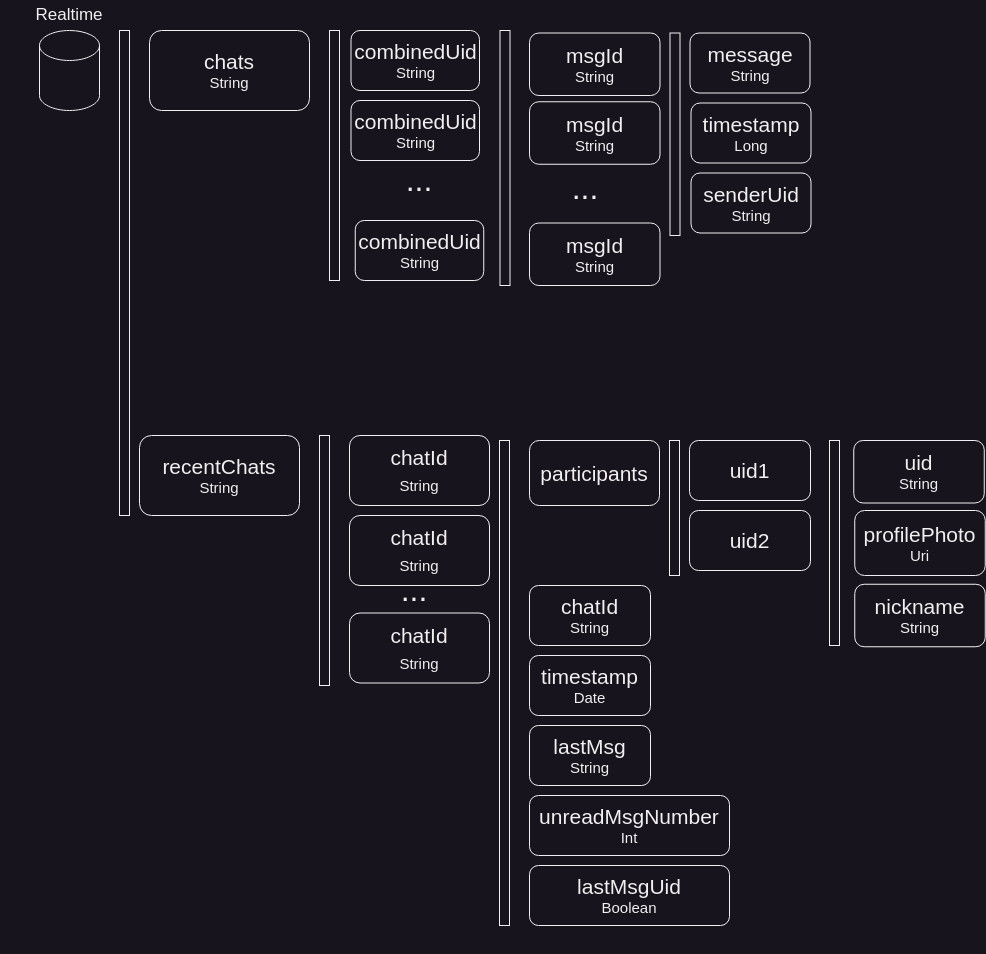
\includegraphics[width = 0.9\textwidth]{Imagenes/drawio/realtime_db.jpg}
	\caption{Diseño de la base de datos Realtime usando Drawio.}
	\label{fig:realtime_db}
\end{figure}

\begin{figure}[ht]
	\centering
	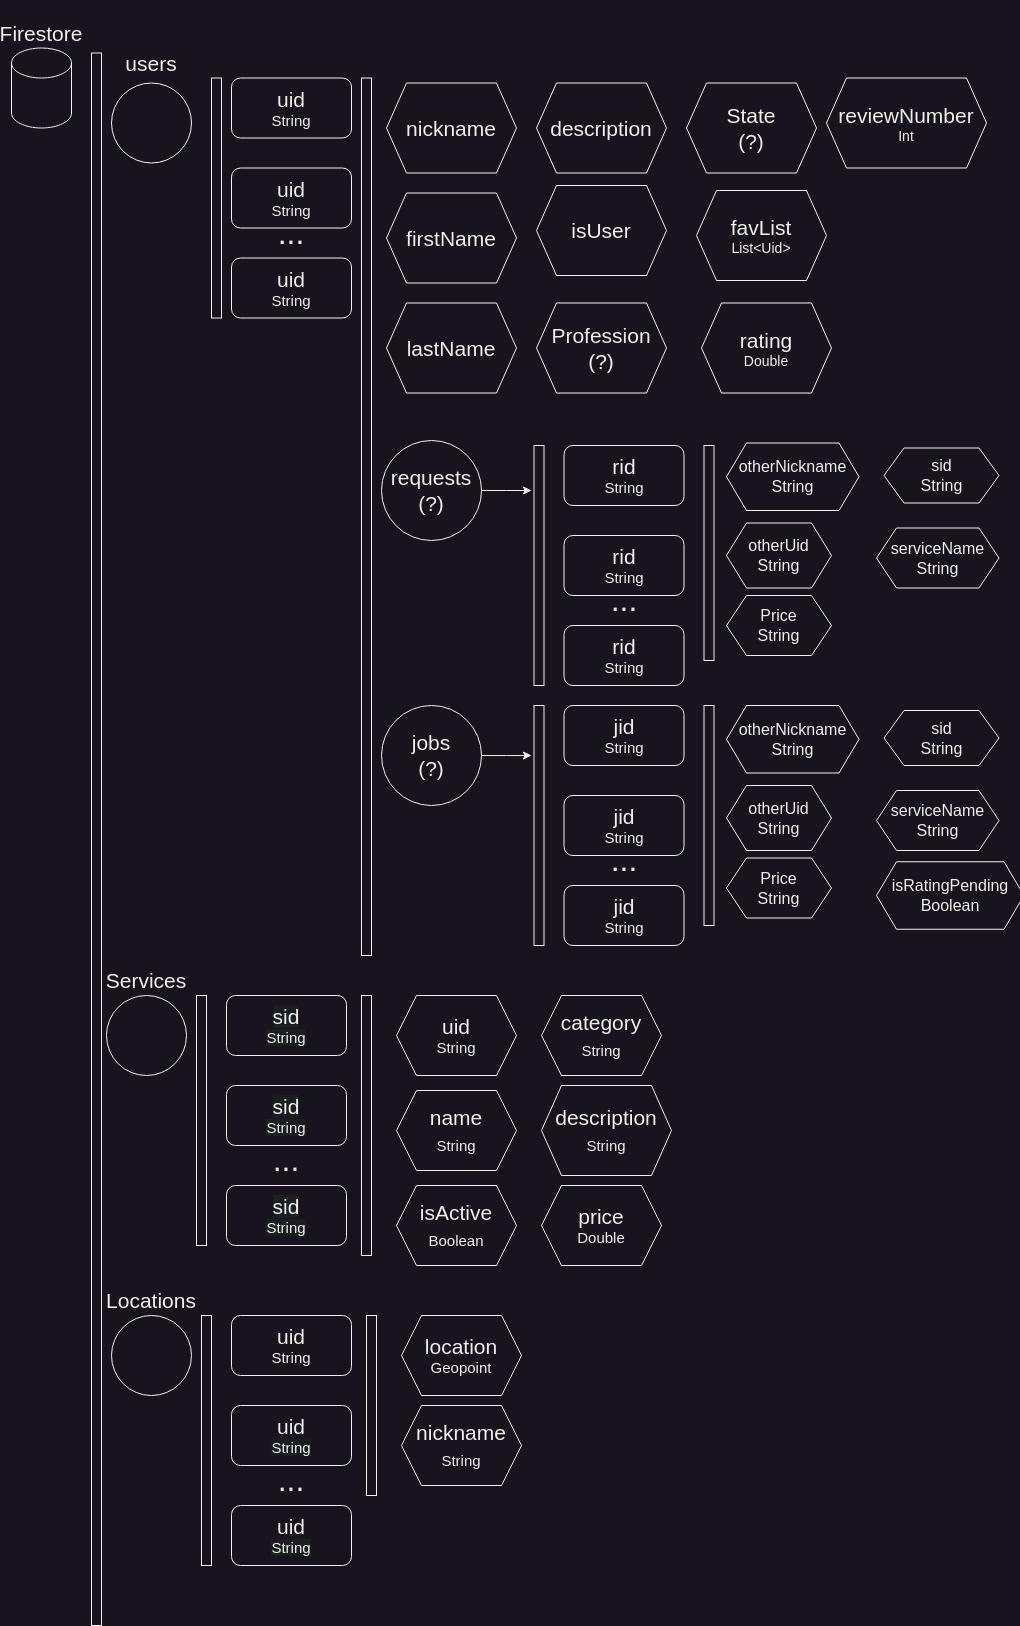
\includegraphics[width = 0.9\textwidth]{Imagenes/drawio/firestore_db.png}
	\caption{Diseño de la base de datos Firestore usando Drawio.}
	\label{fig:firestore_db}
\end{figure}
\chapter{Interfaces de Profinder diseñadas en figma}
\label{Appendix:interfacesfigma}
En este apéndice, se han adjuntado capturas de los diseños de pantallas en \hyperlink{subsec:figma}{Figma}. El proyecto se puede ver aquí: \href{https://www.figma.com/file/RczHTTSY0EkrdOnrnHMPWb/Profinder?type=design&node-id=0%3A1&mode=design&t=BnrHPXS7PUtcqHPP-1}{Link al proyecto}.
\begin{figure}[h]
	\centering
	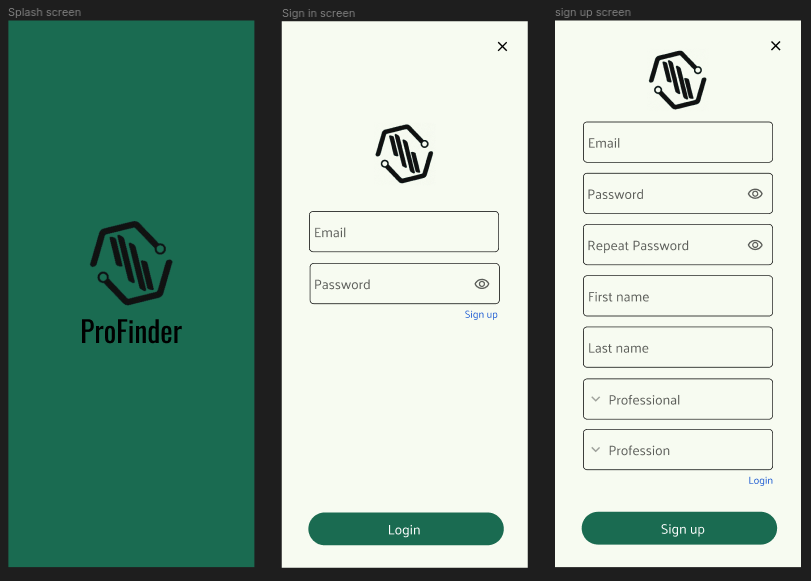
\includegraphics[width = 1\textwidth]{Imagenes/figma/figma1.png}
	\caption{Splash Screen, Login Screen y Sing Up Screen.}
	\label{fig:figma1}
\end{figure}
\begin{figure}[h]
	\centering
	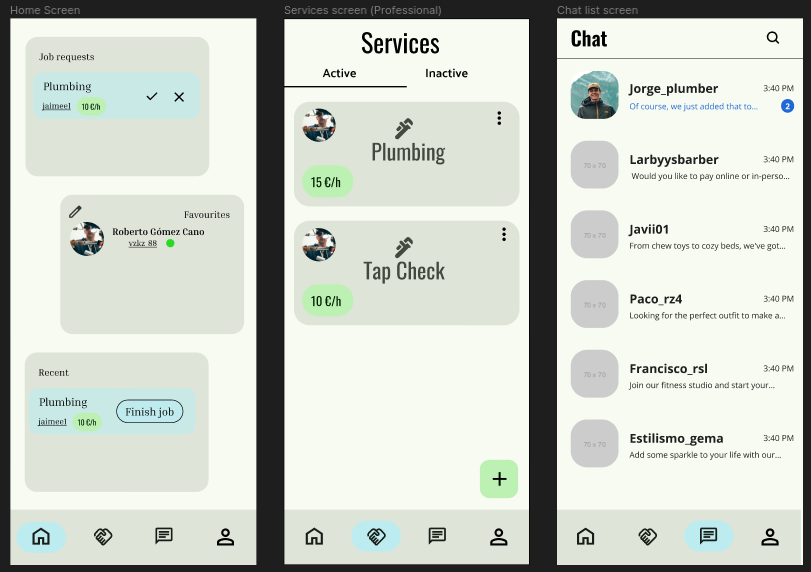
\includegraphics[width = 1\textwidth]{Imagenes/figma/figma2.png}
	\caption{Home Screen, Services Screen (professional) y Chat Screen.}
	\label{fig:figma2}
\end{figure}
\begin{figure}[h]
	\centering
	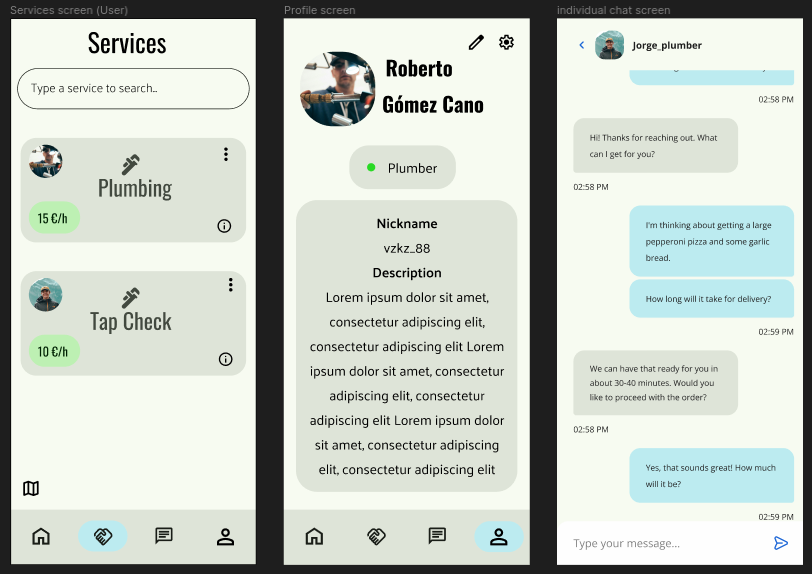
\includegraphics[width = 1\textwidth]{Imagenes/figma/figma3.png}
	\caption{Services Screen (user), Profile Screen y Individual Chat Screen.}
	\label{fig:figma3}
\end{figure}
% \chapter{URLs referenciadas en la memoria}
\label{Appendix:urls}
\begin{itemize}
  \item Uber: \url{https://www.uber.com}
  \item Habitissimo: \url{https://www.habitissimo.es}
  \item Booksy: \url{https://booksy.com/en-us}
  \item Upwork: \url{https://www.upwork.com}
  \item Introducción a Android Views: \url{https://www.studytonight.com/android/introduction-to-views}
  \item Android Studio: \url{https://developer.android.com/studio/intro}
  \item Intellij Idea: \url{https://www.jetbrains.com/idea}
  \item Java: \url{https://www.java.com}
  \item Scala: \url{https://www.scala-lang.org}
  \item Obsidian: \url{https://obsidian.md}
  \item Figma: \url{https://www.figma.com}
  \item Material Design: \url{https://m3.material.io}
  \item Drawio: \url{https://www.drawio.com/}
  \item Mockk Android: \url{https://mockk.io/ANDROID.html}
  \item Git: \url{https://git-scm.com/}
  \item Github: \url{https://github.com/}
  \item Lazygit: \url{https://github.com/jesseduffield/lazygit}
  \item Kotlin: \url{https://kotlinlang.org/}
  \item What is Kotlin: \url{https://www.plainconcepts.com/es/kotlin-android/}
  \item Jetpack Compose: \url{https://developer.android.com/develop/ui/compose}
  \item Lambdas en Kotlin: \url{https://kotlinlang.org/docs/lambdas.html}
  \item Dagger Hilt: \url{https://dagger.dev/hilt/}
  \item Android SDK for Maps: \url{https://developers.google.com/maps/documentation/android-sdk}
  \item Android Maps Compose: \url{https://github.com/googlemaps/android-maps-compose}
  \item Compose Destinations: \url{https://github.com/raamcosta/compose-destinations}
  \item Coil: \url{https://coil-kt.github.io/coil/compose/}
  \item Glide: \url{https://github.com/bumptech/glide}
  \item Picasso: \url{https://square.github.io/picasso/}
  \item Free Software Foundation: \url{https://www.fsf.org/}
  \item GNU: \url{https://www.gnu.org/}
  \item Firefox: \url{https://www.mozilla.org/es-ES/firefox/}
  \item Neovim: \url{https://neovim.io/}
  \item Linux: \url{https://www.linux.org/pages/}
  \item Viewmodel: \url{https://developer.android.com/topic/libraries/architecture/viewmodel}
  \item Patrón MVVM: \url{https://builtin.com/software-engineering-perspectives/mvvm-architecture}
  \item Android Intent: \url{https://developer.android.com/guide/components/intents-filters}
  \item Vídeo Phillip Lackner sobre gestión de errores: \url{https://www.youtube.com/watch?v=MiLN2vs2Oe0}
  \item Expresiones When en Kotlin: \url{https://kotlinlang.org/docs/control-flow.html#when-expression}
  \item Biblioteca Compose Shimmer: \url{https://github.com/valentinilk/compose-shimmer}
  \item Kotlin multiplatform: \url{https://kotlinlang.org/docs/multiplatform.html}
\end{itemize}


%\include{...}
%\include{...}
\backmatter



%
% Índice de palabras
%

% Sólo  la   generamos  si  está   declarada  \generaindice.  Consulta
% TeXiS.sty para más información.

% En realidad, el soporte para la generación de índices de palabras
% en TeXiS no está documentada en el manual, porque no ha sido usada
% "en producción". Por tanto, el fichero que genera el índice
% *no* se incluye aquí (está comentado). Consulta la documentación
% en TeXiS_pream.tex para más información.
\ifx\generaindice\undefined
\else
%%---------------------------------------------------------------------
%
%                        TeXiS_indice.tex
%
%---------------------------------------------------------------------
%
% TeXiS_indice.tex
% Copyright 2009 Marco Antonio Gomez-Martin, Pedro Pablo Gomez-Martin
%
% This file belongs to TeXiS, a LaTeX template for writting
% Thesis and other documents. The complete last TeXiS package can
% be obtained from http://gaia.fdi.ucm.es/projects/texis/
%
% This work may be distributed and/or modified under the
% conditions of the LaTeX Project Public License, either version 1.3
% of this license or (at your option) any later version.
% The latest version of this license is in
%   http://www.latex-project.org/lppl.txt
% and version 1.3 or later is part of all distributions of LaTeX
% version 2005/12/01 or later.
%
% This work has the LPPL maintenance status `maintained'.
% 
% The Current Maintainers of this work are Marco Antonio Gomez-Martin
% and Pedro Pablo Gomez-Martin
%
%---------------------------------------------------------------------
%
% Contiene  los  comandos  para  generar  el índice  de  palabras  del
% documento.
%
%---------------------------------------------------------------------
%
% NOTA IMPORTANTE: el  soporte en TeXiS para el  índice de palabras es
% embrionario, y  de hecho  ni siquiera se  describe en el  manual. Se
% proporciona  una infraestructura  básica (sin  terminar)  para ello,
% pero  no ha  sido usada  "en producción".  De hecho,  a pesar  de la
% existencia de  este fichero, *no* se incluye  en Tesis.tex. Consulta
% la documentación en TeXiS_pream.tex para más información.
%
%---------------------------------------------------------------------


% Si se  va a generar  la tabla de  contenidos (el índice  habitual) y
% también vamos a  generar el índice de palabras  (ambas decisiones se
% toman en  función de  la definición  o no de  un par  de constantes,
% puedes consultar modo.tex para más información), entonces metemos en
% la tabla de contenidos una  entrada para marcar la página donde está
% el índice de palabras.

\ifx\generatoc\undefined
\else
   \addcontentsline{toc}{chapter}{\indexname}
\fi


% Generamos el índice
\printindex

% Variable local para emacs, para  que encuentre el fichero maestro de
% compilación y funcionen mejor algunas teclas rápidas de AucTeX

%%%
%%% Local Variables:
%%% mode: latex
%%% TeX-master: "./tesis.tex"
%%% End:

\fi

%
% Lista de acrónimos
%

% Sólo  lo  generamos  si  está declarada  \generaacronimos.  Consulta
% TeXiS.sty para más información.


\ifx\generaacronimos\undefined
\else
%---------------------------------------------------------------------
%
%                        TeXiS_acron.tex
%
%---------------------------------------------------------------------
%
% TeXiS_acron.tex
% Copyright 2009 Marco Antonio Gomez-Martin, Pedro Pablo Gomez-Martin
%
% This file belongs to TeXiS, a LaTeX template for writting
% Thesis and other documents. The complete last TeXiS package can
% be obtained from http://gaia.fdi.ucm.es/projects/texis/
%
% This work may be distributed and/or modified under the
% conditions of the LaTeX Project Public License, either version 1.3
% of this license or (at your option) any later version.
% The latest version of this license is in
%   http://www.latex-project.org/lppl.txt
% and version 1.3 or later is part of all distributions of LaTeX
% version 2005/12/01 or later.
%
% This work has the LPPL maintenance status `maintained'.
% 
% The Current Maintainers of this work are Marco Antonio Gomez-Martin
% and Pedro Pablo Gomez-Martin
%
%---------------------------------------------------------------------
%
% Contiene  los  comandos  para  generar  el listado de acrónimos
% documento.
%
%---------------------------------------------------------------------
%
% NOTA IMPORTANTE:  para que la  generación de acrónimos  funcione, al
% menos  debe  existir  un  acrónimo   en  el  documento.  Si  no,  la
% compilación  del   fichero  LaTeX  falla  con   un  error  "extraño"
% (indicando  que  quizá  falte  un \item).   Consulta  el  comentario
% referente al paquete glosstex en TeXiS_pream.tex.
%
%---------------------------------------------------------------------


% Redefinimos a español  el título de la lista  de acrónimos (Babel no
% lo hace por nosotros esta vez)

\def\listacronymname{Lista de acrónimos}

% Para el glosario:
% \def\glosarryname{Glosario}

% Si se  va a generar  la tabla de  contenidos (el índice  habitual) y
% también vamos a  generar la lista de acrónimos  (ambas decisiones se
% toman en  función de  la definición  o no de  un par  de constantes,
% puedes consultar config.tex  para más información), entonces metemos
% en la  tabla de contenidos una  entrada para marcar  la página donde
% está el índice de palabras.

\ifx\generatoc\undefined
\else
   \addcontentsline{toc}{chapter}{\listacronymname}
\fi


% Generamos la lista de acrónimos (en realidad el índice asociado a la
% lista "acr" de GlossTeX)

\printglosstex(acr)

% Variable local para emacs, para  que encuentre el fichero maestro de
% compilación y funcionen mejor algunas teclas rápidas de AucTeX

%%%
%%% Local Variables:
%%% mode: latex
%%% TeX-master: "../Tesis.tex"
%%% End:

\fi

%
% Final
%
% %---------------------------------------------------------------------
%
%                      fin.tex
%
%---------------------------------------------------------------------
%
% fin.tex
% Copyright 2009 Marco Antonio Gomez-Martin, Pedro Pablo Gomez-Martin
%
% This file belongs to the TeXiS manual, a LaTeX template for writting
% Thesis and other documents. The complete last TeXiS package can
% be obtained from http://gaia.fdi.ucm.es/projects/texis/
%
% Although the TeXiS template itself is distributed under the 
% conditions of the LaTeX Project Public License
% (http://www.latex-project.org/lppl.txt), the manual content
% uses the CC-BY-SA license that stays that you are free:
%
%    - to share & to copy, distribute and transmit the work
%    - to remix and to adapt the work
%
% under the following conditions:
%
%    - Attribution: you must attribute the work in the manner
%      specified by the author or licensor (but not in any way that
%      suggests that they endorse you or your use of the work).
%    - Share Alike: if you alter, transform, or build upon this
%      work, you may distribute the resulting work only under the
%      same, similar or a compatible license.
%
% The complete license is available in
% http://creativecommons.org/licenses/by-sa/3.0/legalcode
%
%---------------------------------------------------------------------
%
% Contiene la última página
%
%---------------------------------------------------------------------


% Ponemos el marcador en el PDF
\ifpdf
   \pdfbookmark{Fin}{fin}
\fi

\thispagestyle{empty}\mbox{}

Este texto se puede encontrar en el fichero Cascaras/fin.tex. Si deseas eliminarlo, basta con comentar la línea correspondiente al final del fichero TFGTeXiS.tex.

\vspace*{4cm}

\small

\hfill \emph{--¿Qué te parece desto, Sancho? -- Dijo Don Quijote --}

\hfill \emph{Bien podrán los encantadores quitarme la ventura,}

\hfill \emph{pero el esfuerzo y el ánimo, será imposible.}

\hfill 

\hfill \emph{Segunda parte del Ingenioso Caballero} 

\hfill \emph{Don Quijote de la Mancha}

\hfill \emph{Miguel de Cervantes}

\vfill%space*{4cm}

\hfill \emph{--Buena está -- dijo Sancho --; fírmela vuestra merced.}

\hfill \emph{--No es menester firmarla -- dijo Don Quijote--,}

\hfill \emph{sino solamente poner mi rúbrica.}

\hfill 

\hfill \emph{Primera parte del Ingenioso Caballero} 

\hfill \emph{Don Quijote de la Mancha}

\hfill \emph{Miguel de Cervantes}


\newpage
\thispagestyle{empty}\mbox{}

\newpage

% Variable local para emacs, para  que encuentre el fichero maestro de
% compilación y funcionen mejor algunas teclas rápidas de AucTeX

%%%
%%% Local Variables:
%%% mode: latex
%%% TeX-master: "../Tesis.tex"
%%% End:

%\end{otherlanguage}
\end{document}
